\documentclass{report}

\usepackage[utf8]{inputenc}
\usepackage{amsmath}
\usepackage{amssymb}
\usepackage{amsthm}
\usepackage{amsfonts}
\usepackage{hyperref}
\usepackage{graphicx}
\usepackage{physics}
\usepackage{enumerate}
\graphicspath{{images/}}
\usepackage[margin=1in]{geometry}
\usepackage{fancyhdr}
\lhead{\sffamily{Quantum Computation}}
\chead{\sffamily{\thepage}}
\rhead{\sffamily{Pradipta Bora}}
\cfoot{}
\numberwithin{equation}{section}
\theoremstyle{definition}
\newcommand{\Mod}[1]{\ (\mathrm{mod}\ #1)}
\newtheorem{theorem}{Theorem}
\newtheorem{lemma}[theorem]{Lemma}
\newtheorem{corollary}[theorem]{Corollary}
\newtheorem{definition}{Definition}
\numberwithin{definition}{section}
\numberwithin{theorem}{section}
\newtheorem{postulate}{Postulate}
\newtheorem*{thesis}{Thesis}
\newtheorem{exercise}{Exercise}
\newtheorem*{example}{Example}

\theoremstyle{remark}
\numberwithin{exercise}{section}
\newtheorem*{solution}{Solution}
\pagestyle{fancy}

\setlength\parindent{0pt}
\title{Quantum Computing and Quantum Information Theory}
\author{Pradipta Parag Bora}
\date{April 2020}

\begin{document}

\begin{titlepage}
    \begin{center}
        \vspace*{1cm}
            
        \Huge
        \textbf{Summer of Science}
            
        \vspace{0.5cm}
        \LARGE
        Quantum Computation
            
        \vspace{1.5cm}
            
        \textbf{Pradipta Parag Bora}
            
        
       
            
        \vspace{0.8cm}
            
        % \includegraphics[width=0.4\textwidth]{university}
            
        \Large
        Mentor: Thariq Shanavas \\
        Roll No: 190050089 \\
        Department Of Computer Science and Engineering
        
        \vspace{2.0cm}
        \begin{figure}[htp]
        \centering
        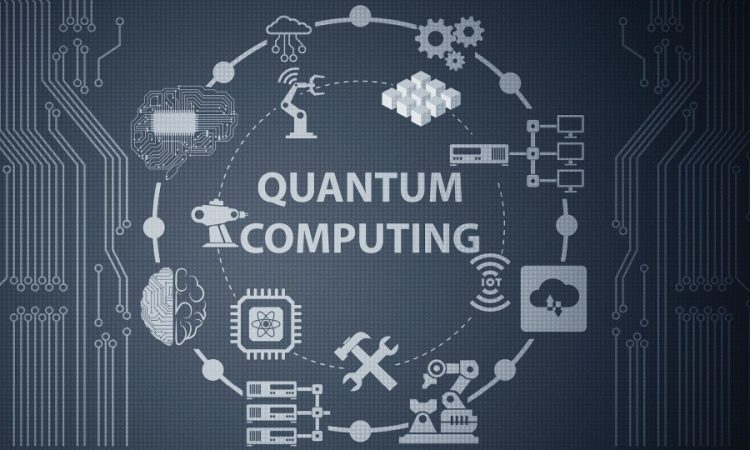
\includegraphics[scale=0.6]{qcom}
    \end{figure}
            
    \end{center}
\end{titlepage}

\tableofcontents

\part{Preliminaries}
\chapter{Introduction}
Through this Summer of Science report, we attempt to summarise everything we covered related to quantum computing and quantum information theory. We will mainly follow the book \textbf{Quantum Computation and Quantum Information} by \textbf{Nielsen and Chuang}. We will begin by going through the mathematical preliminaries, including an introduction to the linear algebraic treatment of quantum mechanics through which we will explore quantum computation. Then we will move onto qubits, their representation and on the way we will study and go through various fascinating quantum algorithms and their uses. Hopefully through this report one will be able to gain a decent understanding of quantum computation. 

The first two sections do not deal with quantum computation and quantum mechanics and instead provide a brief overview of the mathematics that we will require along with the basic ideas of computer science. We then move onto the postulates of quantum mechanics and then we start with basic quantum circuits. Once we have built an understanding of the basics we will go through several quantum algorithms starting with relatively simple ones and ending with quantum fourier transform and quantum search.
\clearpage
\chapter{Mathematical Preliminaries}

We assume that the reader is familiar with basic linear algebra that is covered during the first year. As our treatment of quantum computation heavily uses this, we will summarise some key theorems and notations that we will be using. The reader is free to skip this section as it merely summarises the mathematical tools that we will use. Also note that the following section is very direct and rarely provides any motivation behind the definitions and results to keep it concise and simply provides a list of the preliminaries. Readers are advised to refer to various references of linear algebra to get a better understanding.

\section{Vectors and Vector Spaces}
The most important structure in linear algebra is a vector which we will represent as $\ket{\psi}$. This vector resides in a vector space that satisfies some axioms that give this structure its core defining properties. This representation of a vector is famously known as the \textit{bra-ket} notation and the $\ket{.}$ is used to represent a vector. The same vector in the vector space $\mathbb{C}^{n}$ is conveniently represented as a column vector.

We will be generally working in the vector space $\mathbb{C}^{n}$ over the field $\mathbb{C}$.
A set of vectors $\ket{\psi_{1}}, \ket{\psi_{2}} \cdots \ket{\psi_{n}}$ is said to be \textit{linearly-independent} if for any set of coefficients ${a_i}$, 
$$\sum_{i=1}^{n} a_i\ket{\psi_{i}} = 0 \implies a_i = 0 \:  \forall   1 \leq i \leq n$$
A set of vectors ${\ket{\psi_{i}}}$ is said to be a spanning set of a vector space $\textbf{W}$ if any vector in $\textbf{W}$ can be represented as a linear combination of that set. Note that such a set may be non-finite however we will be dealing with finite dimensional vector spaces only. If this set is linearly independent then this set is called a \textit{basis} of that vector space. It is left as an exercise to show that the cardinality of all bases are same and this value is termed as the \textit{dimension} of that vector space.

\section{Linear Operators and Matrices}
A linear operator $A$ from vector space \textbf{V} to \textbf{W} is a function mapping vectors from \textbf{V} to \textbf{W} satisfying linearity, that is:
$$ A(\sum_{i} a_i \ket{\psi_{i}}) = \sum_{i} a_{i}A\ket{\psi_{i}} $$ 
We can then define compositions of operators, $BA$ as function that first operates $A$ and then operates $B$. 

It is easy to see that matrix multiplication is a linear operator. Conversely any linear operator has a matrix representation. To see this, let $A: V \to W$ be a linear operator. Let $\ket{v_{i}}$ be an ordered basis (basis formed by fixing order of its elements, in this case by enforcing an order restriction on $\ket{v_{i}}$.) of $V$ and $\ket{w_{j}}$ be an ordered basis of $W$.

Then there exists complex numbers $A_{i,j}$ such that: $$A\ket{v_{i}} = \sum_{j} A_{i,j}\ket{w_{j}}$$
If we represent any vector in $V$ by its coordinate vector representation, that is form a column vector whose elements with respect to an ordered basis are the scalar coefficients along the basis elements  and multiply it by the matrix formed by $A_{i,j}$ we get the coordinate vector representation of the output vector in the ordered basis $\ket{w_{j}}$.

\section{Inner Products}
An inner product of a vector space \textbf{V} is defined as a function from $\textbf{V} \cross \textbf{V}$ to $\textbf{C}$. We will denote the inner product of $\ket{v}$ and $\ket{w}$ as $(\ket{v}, \ket{w})$ or as $\braket{v}{w}$. The inner product satisfies the following properties:
\begin{enumerate}
    \item $\braket{v}{w} = ({\braket{w}{v}})^{*}$
    \item $\braket{v}{\sum_{j} a_{j} \ket{w_{j}}} = \sum_{j} a_{j} \braket{v}{w_{j}}$
    \item $\braket{v}{v} \geq 0 $ with equality \textit{iff} $v=0$
\end{enumerate}
We can now define the \textit{length} or \textit{norm} of a vector 
$\norm{\ket{v}} = \sqrt{\braket{v}{v}}$. 
Two vectors are said to be orthogonal if their inner product is $0$. 
We now define an \textit{orthonormal} basis as a basis $\ket{v_{i}}$ whose elements have unit norm and they are pairwise orthogonal, that is for $i\neq j \braket{v_i}{v_j} = 0$.
It can be proven that every finite dimensional vector space has an orthonormal basis. This is left as an exercise. The procedure for determining this orthonormal set from any basis is termed as the \textit{Gram-Schmidt} orthogonalisation process.


This leads to a simple representation of the inner products of two vectors in matrix form. Let $\ket{w} = \sum_i w_i \ket{i}$ and $\ket{v} = \ket{v} = \sum_j v_j \ket{j} $ be two vectors written with the same orthogonal basis.
Then $\braket{w}{v} = (\sum_i w_i \ket{i}, \sum_j v_j \ket{j}) = \sum_i w_{i}^*v_i  $ which we can nicely write in matrix form as
$$ \begin{bmatrix} v_1^* & v_2^* & \cdots & v_n^* \end{bmatrix} \begin{bmatrix} w_1 \\ w_2 \\ \vdots \\ w_n \end{bmatrix}$$

We now introduce the outer product notation. Take two vectors $\ket{w} $ and $\ket{v}$ belonging to inner product spaces. Define the outer product between them to be the linear operator $\ket{w}\bra{v}$ which operates on $\ket{v_'}$ belonging to the same vector space as $\ket{v}$ yielding:
$$ (\ket{w}\bra{v})\ket{v_'} = \braket{v}{v_'}\ket{w} $$
One use of this can be seen as follows:

Let $\ket{i}$ be an orthonormal basis of a vector space $\textbf{V}$. Then for any vector $\ket{v}$ in this vector space, it is easy to see that 
$$(\sum_i \ket{i}\bra{i}) \ket{v} = \ket{v}$$
which in turn implies that $$\sum_i \ket{i}\bra{i}) = I_v $$
This is termed as the completeness relation.

Using this we can easily get the matrix representation of an operator $A: \textbf{V} \to \textbf{W}$. Let $\ket{v_i}$ be an orthonormal basis for $\textbf{V}$ and $\ket{w_j}$ be an orthonormal basis for $\textbf{W}$
$$A = I_{W}AI_{V} = \sum_{i, j} \ket{w_j}\bra{w_j}A\ket{v_i}\bra{v_i}$$
The terms $\bra{w_j}A\ket{v_i}$ are nothing but the entries of the matrix corresponding to this transformation written in coordinate vector form.

\section{Eigenvalues and Eigenvectors}
An eigenvector for a linear operator $A$ is a non-zero vector $\ket{v}$ such that $A\ket{v} = v\ket{v}$ for some complex number $v$. This number is called the eigenvalue corresponding to this eigenvector and we will refer to both the eigenvalue and the eigenvalue by the same letter.

A sufficient and necessary condition for a number $\lambda$ to be an eigenvalue is $$\det|A-\lambda I| = 0$$
We will term the subspace spanned by eigenvectors corresponding to the same eigenvalue as the eigenspace corresponding to that eigenvalue.
Now we introduce diagonalizable operators. An operator is said to be diagonalizable on a vector space if there exists an orthonormal basis composed of eigenvectors of that operator. It is left as an exercise to show that such an operator $A$ can be represented as:
$$ A = \sum_i \lambda_i \ket{i}\bra{i} $$ where $\ket{i}$ corresponds to the orthonormal eigenvectors and $\lambda_i$ are the corresponding eigenvalues.
We will now look at some conditions under which operators are diagonalizable. This is of importance to us as we will be using the diagonal representation of the operator many times later on.

\section{Adjoints and Hilbert Spaces}

For any linear operator $A$ it can be proven that there is a unique linear operator $A^{\dagger}$ satisfying 
$$ (\ket{w}, A\ket{v}) = (A^{\dagger}\ket{w}, \ket{v})$$
This operator is termed as the adjoint of $A$.
It can be shown that the matrix representation of $A^\dagger$ is obtained by taking the complex conjugate and then the transpose of $A$ or $A^\dagger = (A^*)^T$.

\begin{definition}
An operator is said to be \textbf{Hermitian} if $A^\dagger = A$.
\end{definition}
We proceed to show an example of an useful hermitian operator, the Projector.
Let $\textbf{W}$ be a $d$ dimensional subspace of $\textbf{V}$ which is $k$ dimensional. Let $\ket{v_1} \cdots \ket{v_d}$ be an orthonormal basis of $\textbf{W}$. By Gram Schmidt process we can extend this to an orthonormal basis of $\textbf{V}$.
The Projector $P: \textbf{V} \rightarrow \textbf{W}$ is defined as:
$$P = \sum_{i=1}^{d} \ket{v_i}\bra{v_i}$$
Informally this projector projects vectors from $\textbf{V}$ to $\textbf{W}$ as it only leaves those components of the vector that are along the basis vectors which are in $\textbf{W}$. We leave some trivial exercises corresponding to the Projector below that can be done by following the definitions.

\begin{exercise}
Prove that $P$ is Hermitian
\end{exercise}
\begin{exercise}
Prove that $P^2 = P$ and thus $P^\dagger P = P$
\end{exercise}
\begin{definition}
An operator is $A$ said to be \textbf{normal} if $A^\dagger A  = AA^\dagger$.
\end{definition}
The following theorem is incredibly useful and we omit its proof as it is rather involved:
\begin{theorem}[Spectral Theorem] An operator A is diagonalizable if and only if it is normal.
\end{theorem}

Now we talk about a special type of normal operators, unitary operators. These operators are of particular interest to us as all single quantum gates can be represented as unitary operators. 
\begin{definition}
An operator is $A$ said to be \textbf{unitary} if $A^\dagger A  = I$.
\end{definition}

A special class of hermitian operators is of particular interest to us. These operators called positive operators are useful as they come up in the polar and singular decompositions which we will discuss shortly.
\begin{definition}
An operator is $A$ said to be \textbf{positive} if $(\ket{v}, A\ket{v}) \in \mathbb{R}^{+}$ for all $\ket{v}$
\end{definition}

Please go through the following exercises related  to positive operators.
\begin{exercise}
Prove that for any operator $A$, $AA^\dagger$ is positive.
\end{exercise}
\begin{exercise}
Prove that any positive operator is necessarily hermitian.
\end{exercise}
\begin{solution}
Let  $A$ be a positive operator. Observe that we can write  $A$ as:
$$ A = \frac{A+A^\dagger}{2} + i\frac{A-A^\dagger}{2i}$$
Observe that $\frac{A+A^\dagger}{2}$ and $\frac{A-A^\dagger}{2i}$ are both hermitian operators. We will call them $B$ and $C$ from now on.

$$(\ket{v}, A\ket{v}) = (\ket{v}, B\ket{v}) + i(\ket{v}, C\ket{v})$$
Observe that for any hermitian operator $B$, 
$$ (\ket{v}, B\ket{v}) \in \mathbb{R}$$
Thus it follows that $ (\ket{v}, C\ket{v}) = 0$ for all $\ket{v}$ which implies $C = 0$. Thus $A = B$ and so $A$ is hermitian.
\end{solution}

\section{Operator Functions}
It becomes useful for us to define functions on operators that are normal. Formally if $A$ is a normal operator and its diagonal representation is as follows:
$$ A = \sum_i v_i \ket{v_i}\bra{v_i}$$ 
then we define $$f(A) = \sum_i f(v_i) \ket{v_i}\bra{v_i}$$
It is easy to see that $f(A)$ is uniquely determined which allows us to define things like square roots of positive operators, exponentials of normal operators etc.

\begin{exercise}
If $A$ is a normal operator satisfying $A^2 = I$ then prove that 
$$ \exp(i\theta A) = \cos{\theta}I + i\sin{\theta}A$$
\end{exercise}
\begin{solution}
Observe that the possible eigenvalues are $1$ and $-1$. Let $\ket{v_j}$ be an orthonormal basis of the eigenspace corresponding to the eigenvalue $1$ and $\ket{w_k}$ be the orthonormal basis for the eigenspace corresponding to $-1$. Then, 
$$ A = \sum_j \ket{v_j}\bra{v_j} - \sum_k \ket{w_k}\bra{w_k} $$
From the definition of the exponential for normal matrices,
$$\exp(i\theta A) = \sum_j \exp(i\theta )\ket{v_j}\bra{v_j} + \sum_k \exp(-i\theta)\ket{w_k}\bra{w_k}$$ 
$$ = \cos{\theta}(  \sum_j \ket{v_j}\bra{v_j} + \sum_k \ket{w_k}\bra{w_k}) + i\sin{\theta}( \sum_j \ket{v_j}\bra{v_j} - \sum_k \ket{w_k}\bra{w_k}) =  \cos{\theta}I + i\sin{\theta}A $$ where we have used the completeness relation and the diagonal decomposition of $A$.
\end{solution}
We briefly mention that the notion of trace for a matrix can be extended for operators. This is because the trace satisfies
$$ tr(AB) = tr(BA) $$ for matrices A, B.
Suppose $A^{'}$ is one matrix representation of $A$. Then it is related to another matrix representation by $A^{''}$ by 
$$A^{'} = PA^{''}P^{-1}$$ for some change of basis matrix $P$.
Clearly by the previous  result $tr(A^{'}) = tr(A^{''})$ and so trace of an operator is independent of its matrix representation.

\section{Polar and Singular Value Decompositions}
We omit the proof of the polar decomposition as it is rather involved. The singular value decomposition follows from the polar decomposition.
\begin{theorem} \textbf{Polar Decomposition}
For any linear operator $A$ on a vector space $\textbf{V}$ there exists unitary $U$ and positive $J, K$ such that
$$A = UJ = KU$$ where
$$J = \sqrt{A^\dagger A}, K = \sqrt{AA^\dagger}$$
\end{theorem}

\begin{theorem} \textbf{Singular Decomposition}
For any square matrix $A$ there exists unitary matrices $M, N$ and diagonal matrix $D$ with positive entries such that
$$A = MDN $$
\end{theorem}
\begin{proof}
By the polar decomposition, there exists unitary $U$ and positive $J$ such that 
$$ A = UJ $$
As J is positive, it is diagonalisable, so $$J = T^\dagger DT$$ where the entries of D are the eigenvalues of $J$ which are positive and $T$ is unitary.
Setting $M = UT^\dagger$ and $N = T$ completes the proof.
\end{proof}

We end the mathematical preliminaries at this stage and move onto the basics of computer science where we discuss the basics of the field which would be useful in our study of quantum computation.
\clearpage

\chapter{Introduction to Computer Science}
Our main motivation behind using quantum computation is to provide an improvement over the classical model of computation. In order to do so we must have a proper notion of how we compare two different models of computation. Many classically difficult to solve problems have in principle quantum algorithms that solve these problems with ease. For instance, the factorisation problem of finding the prime factors of a number $N$, takes exponentially more time classically than via the quantum Shor's algorithm. But how do we quantify which algorithm is better or efficient? We will deal with this at the end of this section. We begin by first briefly discussing a model of computation that is deemed to be universal, the Turing model. We then provide a circuit equivalent of the same which is more feasible to us. We then look into how we can compare algorithms and finally end this section by describing different classes of algorithms on the basis of their complexities.

\section{Turing Machines}
The field of computer science arose back in the 1930s when the pioneers of the field Alan Turing and Alonzo Church formalized the notion of an algorithm used to solve mathematical problems by providing a model of computation. Turing's model, called the Turing Machine provides an abstract notion of a machine, that in principle can solve all problems associated with an algorithmic process. We will discuss its construction now.

A Turing machine contains four main elements:
\begin{enumerate}
    \item a program, rather like an ordinary computer which contains the instructions corresponding to the algorithm
    \item a finite state control, which acts like a stripped-down microprocessor working with the other components and containing the states of the machine
    \item a tape which is the memory/output of the machine
    \item a read write tape head, which points to the current position on the tape which is being accessed.
\end{enumerate}

The main component of the turing machine is the finite state control, which contains a collection of states of the machine and the machine works by trying to look for the instruction in this collection that corresponds to the current state the Turing machine is in.
Let the states of the machine be $q_1, q_2 \cdots q_m$ and two other special states $q_s$ and $q_h$ which correspond to the starting and halt state respectively. The machine stops operating whenever $q_h$ is obtained. \\ The tape can be thought of as a linear sequence of squares where each element is either $0, 1, b$ or $s$ where $b$ corresponds to a blank square and $s$ refers to the left most starting square on the tape. The tape will start with $s$ and then contain some zeros and ones and finally have blanks on it. The read write tape head is responsible for pointing at the current square and overwriting it with the new value on the square as the machine moves onto the next square. This can be regarded as both the input and the output of the device. 
\\ Let us see how the turing machine works. We will illustrate this via an example. We'll show an explicit construction of a turing machine that outputs the function $f(x) = 1$.
Firstly let us see how the program of the machine is defined. Formally a \textit{program} in a turing machine is a list of tuples (which correspond to commands) of the form 
$$ \left( q_i, x, q_j, x^{'}, d \right)$$
where $q_i$ is the current state in which the machine is supposed to be, $x$ is the value on the current square in the tape head, $q_j$ is the state the machine goes into after executing the current command, $x'$ is the value that the machine will write on the current square after this command is executed and $d$ is either $0, +1, -1$ where a value of $0$ instructs the machine to not move the tape head, +1 means move the pointer to the right and $-1$ means move the tape to the left. The only exception to this rule is when the current value on the tape is $s$ which would ignore the $-1$ instruction as we are at the beginning of the tape.
\\The machine will obtain its current working condition by reading the value on the tape square and scan for the program line that has its current state and this value as the first two elements of the tuple. If such a line does not exist it automatically goes to $q_h$ and halts execution.
\begin{figure}[htp]
    \centering
    \caption{Structure of a Turing Machine}
    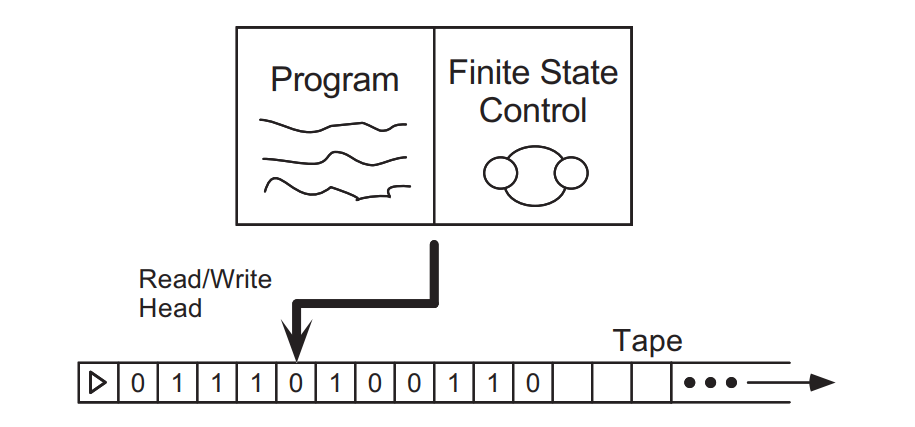
\includegraphics[width=\textwidth]{turing}
\end{figure}
\\ Now we will list an explicit program for computing $f(x)=1$.
Consider the following program:
\begin{enumerate}
    \item $ \left( q_s, s, q_1, s, 1 \right)$
    \item $ \left( q_1, 0, q_1, b, 1 \right)$
    \item $ \left( q_1, 1, q_1, b, 1 \right)$
    \item $ \left( q_1, b, q_2, b, -1 \right)$
    \item $ \left( q_2, b, q_2, b, -1 \right)$
    \item $ \left( q_2, s, q_3, s, 1 \right)$
    \item $ \left( q_3, b, q_h, 1, 0 \right)$
\end{enumerate}

We can see that this program outputs $f(x)=1$ followed by a series of blanks. It is upto you to verify this by tracing the working of the machine line by line.
Although it seems that we certainly did not require such a complex setup to simply compute $f(x) = 1$ the beauty of turing machines lie in the fact that this process can be used to compute various functions ranging from addition, polynomial evaluation to complex arithmetic. Infact all operations that you can do on your current computer can be done on a turing machine. The efficiencies may be different but we are more interested in knowing which problems can indeed be solved on a turing machine.
Church and Turing came up with their thesis, the Church Turing thesis that answers exactly this question.
\begin{thesis}
\textbf{Church Turing Thesis:} The class of functions computable by a Turing machine corresponds exactly to the class of functions which we would naturally regard as being computable by an algorithm.
\end{thesis}
It is to note that this is a hypothesis that has not been proven, however over the last 60 years no counter evidence for the same has been found.
It is interesting to note that quantum computers, and in general, the quantum model of computation do not change the class of functions computable by the model, it merely provides a more efficient way to do so.

Showing that the turing model of computation universally reflects what it means to have an algorithm compute a function is beyond the scope of this report. We will now go through some variations of turing machines. For instance, instead of having just one single tape, the machine could contain two tapes wherein you can use one for the input and other for the output. This variation is identical to the simple turing machine in the sense that both can compute the same set of functions. However for explicitly writing programs for a turing machine it is indeed more convenient to work with the two tape version.
A program line of this turing machine will be of the form $\left(q, x_1, x_2, q^{'}, x_1^{'}, x_2^{'}, d_1, d_2 \right)$ where we will use subscript $1$ for the first tape and $2$ for the other tape.

\begin{exercise}
Write the program lines for a Turing Machine to compute the binary NOT of a binary number provided to you as input in a tape.
(Hint: for such problems it makes more sense to use multiple taped turing machines and more symbols than just $0, 1, b, s$)
\end{exercise}
\begin{exercise}
Describe a Turing program to reverse a binary number provided to you as input in the tape.
\end{exercise}
Another version of a turing machine is a probabilistic turing machine. This machine will transition from one state to another by randomly choosing a state from various possibilities. Note that a deterministic turing machine can in essence simulate a probabilistic machine by going through all possibilities (searching through the search space). Thus they both can compute the exact same class of functions. The probabilistic machine may be more efficient but right now we are only interested in knowing the differences in the set of possible functions computable by different computation models.

Now we describe the circuit model of computation in brief.

\section{Circuit Model of Computation}
The circuit model of computation is essentially the model we are most familiar with, wires and gates that compute binary functions. Taking multiple inputs we can actually compute all kinds of functions which are equivalent to those that can be simulated on a turing machine.  In general our circuits will have gates, which are blocks that compute functions of the form $f : \{0, 1 \}^{k} \to \{0, 1\}^{l}$. However we would like to reduce all our circuits to those made up of some universal blocks. There are a few gates called the universal gates in classical computation that can build up any gate. One such gate is the NAND gate which takes two binary inputs and computes their binary AND and then negates the result.

There are other universal gates as well and some common gates like OR, AND, XOR which are self explanatory. Two other gates are the FANOUT and crossover gates. The FANOUT gate takes an input and copies it out. We will later see that the FANOUT gate has no quantum equivalent because of the \textit{no-cloning} theorem. The crossover gate takes two inputs and simply swaps them.

Later on when we get into quantum circuits, we will show quantum equivalents of these gates and also look at universal quantum gates. It is important to note that quantum mechanics is reversible, infact all of quantum mechanics can be represented as unitary transformations which we will look into in the next section. As a result it is not possible to have irreversible gates in our quantum computational model. So a quantum variant of an AND gate is not possible as AND is irreversible which means that given the output of the AND gate we cannot determine what the inputs were. We reserve this discussion for later when we start dealing with quantum circuits.

\section{Analysis of Computational Problems}

So far we have said that quantum computers provide a more efficient solution of various classical problems. How do we deem which algorithm is better? This section deals with that.

First we talk about orders of magnitude of functions. Let us take an algorithm which scans a list of $n$ numbers and outputs the maximum among them. Clearly such an algorithm takes $n$ operations to finish. In general lesser the number of steps the better the algorithm. But we cannot really talk about the exact number of steps and instead we need an estimate on the number of steps as this value can be variable. Suppose we have an algorithm that scans a list of $n$ numbers to check if $1$ is present or not and if it finds $1$ it terminates. Clearly this can take any number of steps ranging from $1$ to $n$. What we know is that at worst it takes $n$ steps (the upper bound) and in the best case it takes $1$ step (lower bound). So the ideas of upper bound and lower bound on the number of steps provide a rough estimate of how good the algorithm is while average case analysis provide a better picture by accounting for all cases. To talk about such cases in a more formalised manner we use the big-O, big-Omega and big-theta notation.

\begin{definition}
\textbf{Big O} A function $f(n)$ is said to be $O(g(n))$ if there exists some constant c and some $n_0$ such that for all $n \geq n_0$, $$ f(n) \leq cg(n)$$
\end{definition}
An algorithm $A$ is said to have (upper) time complexity $O(g(n))$ if the function $\textbf{TIME}(A(n)) = f(n)$ is $O(g(n))$ where $f(n)$ is the number of steps the algorithm takes on that input.
For example the previous algorithm is $O(n)$ as for $c = 1$ and $n_0 = 1$
$f(n) \leq n$ is satisfied where $n$ is the size of our input.

Similarly we have big theta and big O notations that deal with different bounds.

\begin{definition}
\textbf{Big Theta} A function $f(n)$ is said to be $\Theta (g(n))$ if there exists some constant $c_1, c_2$ and some $n_0$ such that for all $n \geq n_0$, $$c_1g(n) \leq f(n) \leq c_2 g(n)$$
\end{definition}
\begin{definition}
\textbf{Big Omega} A function $f(n)$ is said to be $\Omega (g(n))$ if there exists some constant $c$ and some $n_0$ such that for all $n \geq n_0$ ,$$ c g(n) \leq f(n)$$
\end{definition}

So for instance, the previous algorithm is $\Omega (1)$ and $O(n)$. It is upto you to prove that we cannot have any $\Theta$ bound for this algorithm.
We can also have space complexity where instead of talking about the number of steps, we refer to the number of memory units the program requires. Therefore the previous algorithm has $\Theta (n)$ space complexity as it is using roughly $n$ memory units to store all values (measured as multiples of memory units used to store one number).

Now let us compare the algorithms for prime factorisation. If a number $N$ is given the size of its input is $\log_2 N$. Remember that computer scientists always deal with logarithms to the base 2 as values are stored in binary. So the implicit base is $2$.
Now Shor's algorithm is $O(\log^3 N)$ which is a massive improvement over classical algorithms. A simple trial algorithm is $O(N)$ which becomes exponential in the input size $\log_2 N$. Notice that we are only concerned with the behaviour of the function at large values of the input as computation becomes infeasible only at those limits.

\begin{exercise}
Consider the Merge Sort algorithm. This algorithm can be defined in pseudocode as follows in recursive form (self calling):
\begin{verbatim}
    MERGESORT(List A, SIZE N):
        List B = List A[0, N/2]
        List C = List A[N/2 + 1, N]
        B = MERGESORT(B, N/2) 
        C = MERGESORT(C, N/2)
        A = MERGE(B, C, N/2, N/2)
        return A
\end{verbatim}
The merge function combines the two lists B and C which have half the number of elements that are already sorted and outputs the sorted list formed by combining B and C.

1. Give an $O(N_1 + N_2)$ complexity algorithm for MERGE(List A, List B, Size N_{1}, Size N_{2}).

2. Using the above algorithm write the recursive definition for \textbf{TIME}(List A, Size N) in terms of N. Use this to compute the  time complexity of Merge Sort.
\end{exercise}

\section{Complexity Classes}
\begin{figure}[htp]
    \centering
    \caption{The various complexity classes}
    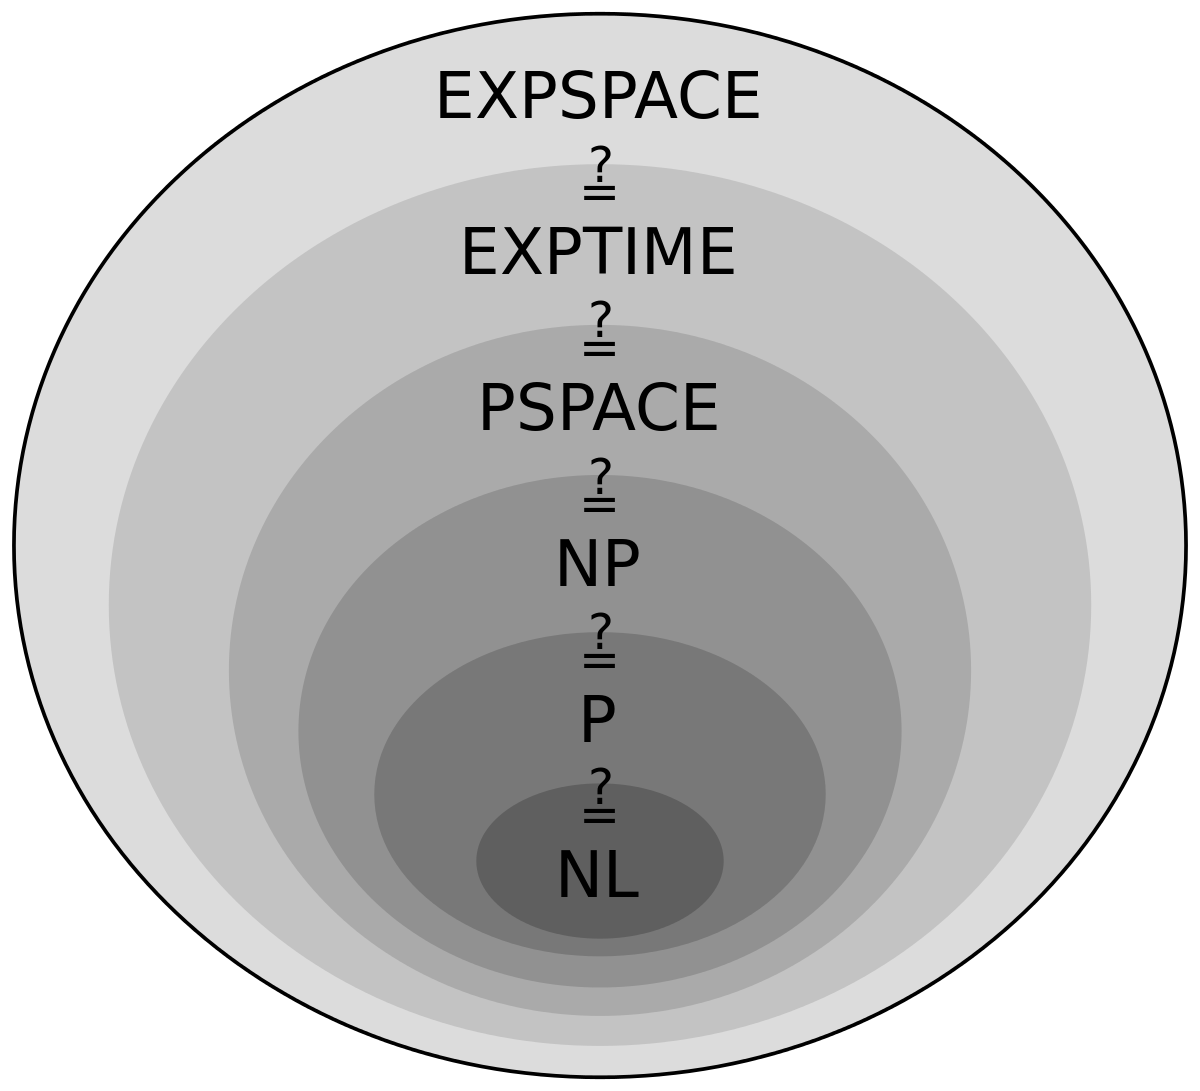
\includegraphics[scale=0.24]{complexity}
\end{figure}
When we covered big-o notation to compare running times of different algorithms we found a way of quantifying the upper bound of the running time. Naturally it makes sense to now categorize different algorithms into different classes on the basis of their running time.

We will start by classifying decision problems, that is problems that have a yes/no answer. These problems provide a lot of insight into the generic case of computable problems and so we stick to them for this report. For instance we may ask the question whether a  number $n$ is a prime or not. This is a decision problem as it has a pure yes/no answer.

To formalize this notion of a decision problem, we rephrase it in terms of a \textit{language} L. A language is a subset of all possible strings formed from a subset of characters which we term as alphabets. For instance we may define the \textit{prime} language $L_P$ as the subset of all possible strings formed from $\{0, 1\}$ such that the corresponding binary number is a prime.

Then we can rephrase decision problems into creating a Turing Machine (or an algorithm) that will output yes if the corresponding input is part of that language and else no. These outputs can be two end states of the turing machine $q_y, q_n$.

A complexity class is a set of problems that satisfy a particular property with respect to its time or space or energy complexity.
For an algorithm (or a machine implementing it) $A$ solving a decision problem $D$ we say that $D \in \textbf{P}$ where \textbf{P} is a complexity class if for an input of size $n$, \textbf{TIME}(A(n)) $ = O(n^k)$ for some $k>0$.
Roughly $\textbf{P}$ is the collection of those decision problems where the decision can be found out in polynomial size of the input.

\textbf{P} is an important complexity class as it contains those problems that we can solve in a reasonable amount of time compared to say exponential or factorial growth algorithms. 

Another important complexity class is \textbf{NP}. Roughly speaking it is that collection of decision problems whose truth value can be verified with the help of another input called the witness W in polynomial size of the main input.
Formally a decision problem is in \textbf{NP} if
\begin{enumerate}
    \item given x $\in $ L, there exists a witness W such that using the W a turing machine can deterministically state that x $\in$ L by going to the positive state $q_y$ in time proportional to a polynomial in size of x.
     \item given x $\not\in $ L, for all possible witnesses W the turing machine will deterministically state that x $\not\in$ L by going to the  state $q_n$ in time proportional to a polynomial in size of x.
\end{enumerate}

For example consider the decision problem $D$ asking whether a number $x$ is \textbf{NOT} in the prime language, that is $ x \in L_P^{'}$ that we previously described. Then a possible witness could be a factor of the number $x$ where we check if the witness divides the number (where the witness is not $x$ or 1). If $x$ was a prime then for any possible witness we cannot use it to say that witness divides the number  and so the second condition is met. Thus this problem is in \textbf{NP}.

In general it is not easy to provide a witness for the complement of a language. For example in the previous case the complement would be the language of primes. There, coming up with a witness that gives a guarantee that $x \in L_P$ is not easy.

\begin{exercise}
Prove that \textbf{P} $\subseteq$ \textbf{NP}
(Hint: it is not necessary to use the witness always)
\end{exercise}
It is not yet known whether  \textbf{P} $\neq$ \textbf{NP} and this is infact a millennium problem. 
There are other complexity classes related in terms of space. \textbf{PSPACE} refers to those problems which take polynomial space while \textbf{EXPSPACE} take exponential space. Similarly we have \textbf{L} for logarithmic time complexity and \textbf{LSPACE} for logarithmic space complexity.

\begin{exercise}
Prove that $\textbf{P} \subseteq \textbf{PSPACE}$
\end{exercise}
With respect to probabilistic turing machines, we have \textbf{BPP} which contains all those decision problems which we can be probabilistically solved in polynomial time with probability atleast $k$ where $k > \frac{1}{2}$. However this $k$ can be made as close to $1$ as we desire by running the algorithm many times for the same input and choosing the maximum occurring result. Thus \textbf{BPP} is more indicative of "fast" solvable problems than \textbf{P} in practice.
We end this section by allauding to another complexity class of particular interest to this, \textbf{BQP}. \textbf{BQP} is the quantum equivalent of \textbf{BPP}, that is those decision problems that can be solved with a high degree of probability $ > \frac{1}{2}$ using a quantum circuit taking time which is polynomial in the size of the input.

\clearpage
\chapter{Postulates of Quantum Mechanics}

We aim to have a self sufficient understanding of Quantum Mechanics and in order to do so we will list the postulates of quantum mechanics in this section and see how they can be useful in our study of quantum computation.

\section{The State Space}
\begin{postulate}
Associated to any isolated physical system is a complex vector space
with inner product (that is, a Hilbert space) known as the state space of the system. The system is completely described by its state vector, which is a unit vector in the system’s state space.
\end{postulate}

This postulate states that any system can be described as a vector spanned by some basis elements. Knowing a basis for our vector space allows us to therefore express the entire system at any point of time in terms of these elements and the transformation of this representation with time is sufficient  for us to describe how the system evolves with time.

It is imperative to note that this postulate merely states the existence and does not provide any knowledge about what this state space is. For this we need to develop additional quantum field theories that model different scenarios. 

Let us take a simple example. We introduce the qubit at this point of time. Classical computers always process data in forms of the bits 0 and 1. But any bit at any point of time can either be 0 or 1. Quantum Computers however allow superposition of these bits.

A qubit can therefore be one of the possible states, that is an element of the state space. The basis elements of this state space are taken as 0 and 1, which we write in vector form as $\ket{0}$ and $\ket{1}$. 
We can therefore write any qubit $\ket{\psi}$ as 
$$\ket{\psi} = a\ket{0} + b\ket{1}$$
The postulate dictates that $\ket{\psi}$ is a unit vector. This ensures that $|a|^2 + |b|^2 = 1$. This must hold even after any transformation is done on the current state vector.

Note that our choice of using $\ket{0}$ and $\ket{1}$ as the basis is arbitary. We can use other bases as well. The basis we use is referred to as the computational basis.

\section{Evolution of the System}
\begin{postulate}
The evolution of a closed quantum system is described by a unitary
transformation. That is, the state $\ket{\psi_1}$ of the system at time $t_1$ is related to the
state $\ket{\psi_2}$ of the system at time $t_2$ by a unitary operator U which depends only on the initial and final time.
$$\ket{\psi_2} = U\ket{\psi_1}$$
\end{postulate}

In our study of quantum computation we will be using various gates. We can consider a gate as a machine that takes in a quantum state and churns out another at a later time. The above postulate thus allows us to model all gates in the form of unitary transformations. It however does not tell us which unitary operators can be used to describe evolution of a system.

It turns out that for quantum gates on a single qubit any unitary operator can be used to describe evolution via a suitable quantum gate.
We describe some gates here in brief. Consider a quantum NOT gate. This must take $\ket{0}$ to $\ket{1}$ and viceversa. This operator is simply:
$$ X = \ket{0}\bra{1} + \ket{1}\bra{0}$$
which in matrix form is simply
$\begin{bmatrix}
0 & 1 \\ 1 & 0
\end{bmatrix}$ \\ \\ 
Similarly we have the phase flip gate Z which takes keeps $\ket{0}$ the same and takes $\ket{1}$ to $-\ket{1}$.
Another useful quantum gate is the Hadamard Gate,
$$ H = \frac{1}{\sqrt{2}}\begin{bmatrix} 1 & 1 \\ 1& -1 \end{bmatrix} $$

\begin{exercise}
Verify that the Hadamard Gate is indeed unitary and find it's eigenvectors and thus diagonalise it.
\end{exercise}

\section{Measurement}
\begin{postulate}
Quantum measurements are described by a collection $\ket{M_m}$ of measurement operators. These are operators acting on the state space of the system being measured. The index $m$ refers to the measurement outcomes that may occur in the experiment. If the state of the quantum system is $\ket{\psi}$ immediately before the measurement then the probability that result $m$ occurs is
$$ p(m) = \bra{\psi}M_m^{\dagger}M_m\ket{\psi} $$
After this measurement the new state vector of the system (given that we obtained $m$) is 
$$ \frac{M_m\ket{\psi}}{\sqrt{\bra{\psi}M_m^{\dagger}M_m\ket{\psi}}} $$
\end{postulate}

These measurement operators must also satisfy the completeness relation as 
$$ \sum_m p(m) = 1$$ which implies $$ \sum_m \bra{\psi}M_m^{\dagger}M_m\ket{\psi} = 1 \implies \sum_m M_m^{\dagger}M_m = I$$

\begin{exercise}
Define a set of Measurement operators that extract the coefficients along the computational basis.
\end{exercise}

This postulate fundamentally describes one of the major features of quantum mechanics, that measurement changes the system. After measuring the state vector collapses into another state.

We now talk about a different way of talking about measurements, the projective measurement operators. Suppose that the act of measurement is denoted by an operator $M$ acting on our state space. Note that this can be done only when your system is closed, or when unitary dynamics can be applied to it (energy is conserved). The act of measurement may change this as external influence is applied.

However assuming energy is conserved than correspondingly $M$ will be unitary and hence will have a spectral decomposition. Moreover as we will be measuring "real" values the eigenvalues will be real and thus $M$ will be hermitian.
Let $m$ refer to the eigenvalues of this observable. Then 
$$ M = \sum_m mP_m $$ 
where $P_m$ is the projector onto the eigenspace corresponding to the eigenvalue $m$. The act of observing the observable $M$ will collapse the state vector into one of the eigenstates. Notice that this is similar to the previous postulates in the special case when our measurement operators are the projectors onto the eigenstates, as if $M_m = P_m$ then $$P_m = M_m^{\dagger}M_m$$
Hence by the previous postulate the probability of getting a value $m$ is 
$$p(m) = \bra{\psi}P_m\ket{\psi}$$ and the state after the measurement is $$\frac{P_{m}\ket{\psi}}{\sqrt{p(m}}$$ The average value of the measurement is then simply $$E(m) = \sum_m mp(m) \\ = \sum_m m\bra{\psi}P_m\ket{\psi} = \bra{\psi}M\ket{\psi}$$

However projective measurements are not all type of measurements. It can be shown that projective measurements along with unitary transformations can account for all measurment operators. We can however make the math corresponding to postulate 3 simpler by invoking a mathematical tool called POVM measurements.

\section{POVM Measurement}

Notice that in Projective measurement the measurement operators were the projectors themselves. As projectors satisifed $P^{\dagger}P = P$ the math corresponding to the probabilities becomes simple. Notice that the only place where we need $M_m$ is to get the state of the system after the measurement. If we do not need or care about this, we can define a new set of operators 
$$E_m = M_m^{\dagger}M_m $$
Then corresponding to $E_m$ there is an eigenvalue $m$ which could be obtained after the measurement. The probability simply becomes
$$p(m) = \bra{\psi}E_m\ket{\psi}$$
and the completeness relation implies 
$$ \sum_m M_m^{\dagger}M_m = \sum_m E_m = I$$
The set of operators $\{E_m\}$ is termed as \textit{POVM} and each $E_m$ is called a \textit{POVM} element. A POVM is sufficient to obtain the probabilities of each measurable value and makes it more elegant reducing the need for adjoints. We have shown that for every set of measurement operators there is a corresponding set of POVMs.

\begin{exercise}
Show that for every POVM there is a corresponding set of Measurement operators.
\end{exercise}
\begin{exercise}
Show that projective measurement operators are a special case of POVMs
\end{exercise}

Note that POVMs and general measurement operators are more general than projective measurements as we do not comment on the nature of the measurement operators. However it can be proven using composite quantum systems that projective measurements along with unitary operators are sufficient to describe any general measurment. We reserve this proof and discussion for a later time.

We briefly mention the final postulate which deals with composite quantum systems. We will revisit this later when we deal with tensor products and partial traces.

\section{Composite Quantum Systems}
\begin{postulate}
The state space of a composite physical system is the tensor product
of the state spaces of the component physical systems. If the state of the ith component is $\ket{\psi_i}$ and total we have $n$ components then the net state is given by 
$$ \ket{\psi_1} \otimes \ket{\psi_2} \otimes \cdots \ket{\psi_n}$$
\end{postulate}

The symbol $\otimes$ is used for the tensor product. We will go through this later when we deal with composite quantum systems in the next section. Essentially tensor products are used to build composite systems out of individual hilbert spaces. Thus we can deal with quantum systems having multiple components like say 3 qubits simultaneously.

We now proceed onto simple quantum circuits. We will start with the most simple case, a quantum gate operating on a single qubit. After we analyse this we will look into tensor products and partial traces in detail which would allow us to analyse multiple qubit gates properly.

\clearpage
\section{Single Qubit Gates}

In this section we will deal with single qubit gates and different ways we can represent them.

A single qubit gate can be represented as an unitary operator acting on the state vector of the qubit.That is for every gate $G$ there exists a unitary transformation $U$ such that the final state of a state vector $\ket{\psi}$ is given by 
$$ \ket{\psi_2} = U\ket{\psi}$$
This is because the gate can be thought of as an abstract machine that takes in a state vector and operates on it with time. As all time transformations of quantum state vectors are unitary transformations the above result holds. Conversely we assume that for every unitary operator on a single qubit there exists a gate for the same. Achieving the construction of such a gate would venture into physical realisation of quantum computation which we reserve for later.

\begin{exercise}
Mathematically prove that all single gate qubit operators have to be unitary by using the normalisation condition of qubit state vectors.
\end{exercise}

We now introduce the bloch sphere notation for qubits. Observe that we can write any qubit as follows:
$$\ket{\psi} = e^{ix}\left(\cos{\frac{\theta}{2}} + ie^{i\phi}\sin{\frac{\theta}{2}}\right)$$ where $$ 0 \leq x < 2\pi,   0 \leq \theta \leq \pi,   0\leq \phi <2\pi$$
\\
The global phase $e^{ix}$ is irrelevant as it is common to both. Observe that by neglecting this our state vector is parameterised by $\theta$ and $\phi$ and these values are precisely in the range of the spherical angular coordinates of a sphere of radius 1. Thus corresponding to every $\ket{\psi}\left(\theta, \phi \right)$ there exists a point on the unit sphere given by $(1, \theta, \phi)$ in spherical polar coordinates.
This sphere is termed as the bloch sphere and the corresponding position vector the bloch vector.\\
It is interesting to note that any unitary transformation in the state space can be visualised to be a rotation of the bloch sphere about an axis. That is this mapping corresponds to a rotation of the bloch sphere (upto a global phase). You will prove this result later on.
We first define some standard gates in their matrix forms. These gates are incredibly useful and are known as the pauli matrices.

$$X = \begin{bmatrix}0&1\\1&0\end{bmatrix}& Y = \begin{bmatrix}0&-i\\i&0\end{bmatrix}&Z=\begin{bmatrix}1&0\\0&-1\end{bmatrix}$$\\

First we would like to describe some standard transformations (or gates) that rotate the sphere about x, y, z axes.

$$R_x(\theta) = e^{-i\theta\frac{X}{2}} = \begin{bmatrix}\cos{\frac{\theta}{2}}& -i\sin{\frac{\theta}{2}}\\-i\sin{\frac{\theta}{2}}&\cos{\frac{\theta}{2}}\end{bmatrix}$$
$$R_y(\theta) = e^{-i\theta\frac{Y}{2}} = \begin{bmatrix}\cos{\frac{\theta}{2}}& -\sin{\frac{\theta}{2}}\\\sin{\frac{\theta}{2}}&\cos{\frac{\theta}{2}}\end{bmatrix}$$
$$R_z(\theta) = e^{-i\theta\frac{Z}{2}} = \begin{bmatrix}e^{\frac{-i\theta}{2}}& 0\\0&e^{i\frac{\theta}{2}}\end{bmatrix}$$

\begin{exercise}
Show that $X^2 = Y^2 = Z^2 = I$ and hence deduce the expansion of their exponentiation as done above using the result of exercise 2.5
\end{exercise}

It is a bit lengthy to show that the above matrices indeed do what we are claiming them to do. You can refer to this \href{http://www.vcpc.univie.ac.at/~ian/hotlist/qc/talks/bloch-sphere-rotations.pdf}{resource} for more detail (you will need to go through density matrices that we introduce in the next section).

It is important to note that in the bloch sphere representation the coefficient along $\ket{0}$ is always a real positive number. After we apply any gate on the state vector this may not be true and so we must first divide by a common phase factor to ensure the above condition is met before we figure out the bloch vector.  

We prove this important theorem that relates unitary transformations to rotation transformations using the rotation matrices.

\begin{theorem}
Suppose U is a unitary transformation. Then there exists reals $\alpha, \beta, \gamma$ and $\delta$ such that 
$$ U = e^{i\alpha}R_z(\beta)R_y(\gamma)R_z(\delta)$$
\end{theorem}

\begin{proof}
Since U is unitary, the rows and columns of U are orthonormal. Thus there exist reals $\alpha, \beta, \gamma$ and $\delta$ such that 
$$U = \begin{bmatrix}e^{i(\alpha - \frac{\beta}{2} - \frac{\delta}{2})}\cos{\frac{\delta}{2}} & -e^{i(\alpha - \frac{\beta}{2} + \frac{\delta}{2})}\sin{\frac{\delta}{2}} \\e^{i(\alpha + \frac{\beta}{2} - \frac{\delta}{2})}\sin{\frac{\delta}{2}}& e^{i(\alpha + \frac{\beta}{2} + \frac{\delta}{2})}\cos{\frac{\delta}{2}}
\end{bmatrix}
$$
By expanding the right hand side of the statement to prove we immediately get the above and thus the given statement is proved.
\end{proof}

The above theorem allows us to construct any gate using just three parameterised gates. There exists an important corollary of the above that we leave as an exercise. This corollary is useful when we want to construct multi qubit gates.

\begin{exercise}
Suppose $U$ is a unitary gate. Show that there exists unitary operators$A, B, C$ on a single qubit such that $ABC=I$ and $U$ is identical to $AXBXC$ upto a global phase.
\end{exercise}

We end this section by mentioning two other important gates that we will later use.
The Hadamard gate was previously introduced and is given by 
$$H = \frac{1}{\sqrt{2}}\begin{bmatrix}1 & 1 \\ 1&-1 \end{bmatrix} $$.
The T gate (also known as the $\frac{\pi}{8}$ gate) is given by 
$$ T = \exp(i\pi/8)\begin{bmatrix} \exp(-i\pi/8) & 0 \\ 0 & \exp(i\pi/8) \end{bmatrix}$$

We will revisit quantum gates in detail later. First let us look into composition of quantum systems and tensor products as we will require this when dealing with multi qubit gates.

\clearpage
\chapter{Composite Quantum Systems}
In this section we will deal with making composite quantum state spaces out of elementary state spaces. This will be important for instance, when we deal with multiple qubits. We begin with tensor products which serve as the mathematical backbone behind composite systems.

\section{Tensor Products}
Suppose \textbf{A} and \textbf{B} are two vector spaces that are $n$ and $m$ dimensional. The tensor product of \textbf{A} and \textbf{B} is denoted as 
$$ \textbf{A} \otimes \textbf{B}$$
This is a vector space that is $nm$ dimensional whose basis elements are the tensor products of the basis elements of the individual vector spaces. An informal way to think of a tensor product is that it is just a placeholder where the individual vector spaces are kept along different dimensions. Suppose $\ket{v} \in \textbf{A}$ and $\ket{w} \in \textbf{B}$, then $$\ket{v} \otimes \ket{w} \in \textbf{A} \otimes \textbf{B}$$.

The tensor product is a vector space and along with that it must satisfy the following properties:
\begin{enumerate}
    \item For scalar $c \in \mathbb{C}$ and $\ket{v} \in \textbf{A}, \ket{w} \in \textbf{B}$ $$c \left(\ket{v} \otimes \ket{w}\right) = c\ket{v}\otimes \ket{w} = \ket{v}\otimes c\ket{w}$$
     \item For $\ket{v_1}, \ket{v_2}  \in \textbf{A}, \ket{w} \in \textbf{B}$ $$ \left(\ket{v_1} + \ket{v_2}\right) \otimes \ket{w} = \ket{v_1}\otimes \ket{w} + \ket{v_2}\otimes \ket{w}$$
      \item For $\ket{v}  \in \textbf{A}, \ket{w_1}, \ket{w_2} \in \textbf{B}$ $$ \ket{v}  \otimes \left(\ket{w_1} + \ket{w_2}\right) = \ket{v}\otimes \ket{w_1} + \ket{v}\otimes \ket{w_2}$$
\end{enumerate}

\begin{exercise}
Using the above axioms prove that if $\ket{i}$ is a basis of $\textbf{A}$ and $\ket{j}$ is a basis of $\textbf{B}$ then $\ket{i} \otimes \ket{j}$ is a basis of $\textbf{A} \otimes \textbf{B}$
\end{exercise}

Similarly we can talk about operators on this tensor space. If $M$ is a linear operator from $\textbf{A} \to \textbf{A}^{'}$ and $N$ is a linear operator from $\textbf{B} \to \textbf{B}^{'}$ then $M \otimes N$ is a linear operator from $\textbf{A} \otimes \textbf{B} \to \textbf{A}^{'} \otimes  \textbf{B}^{'}$ defined by 
$$ \left(M \otimes N \right) \ket{i} \otimes \ket{j} = M\ket{i} \otimes N\ket{j}$$
for $\ket{i} \otimes \ket{j} \in \textbf{A} \otimes \textbf{B}$. It is trivial to show using the above properties that the above operator is indeed linear. This is left as an exercise.

We can also define an inner product on this vector space. Let $\textbf{A}$ be an inner product space and $\textbf{B}$ be an inner product space. Then we define an inner product on $\textbf{A} \otimes \textbf{B}$ by 
$$ (\left \ket{v_1} \otimes \ket{w_1}, \ket{v_2} \otimes \ket{w_2} \right) = (\left \ket{v_1} , \ket{v_2} \right) (\left \ket{w_1}, \ket{w_2} \right) $$ for $\ket{v_1}, \ket{v_2} \in \textbf{A}, \ket{w_1}, \ket{w_2} \in \textbf{B}$. This way two sets of orthonormal bases created an orthonormal base of their tensor product space.

As an example suppose we have two qubits, then this composite system will have the bases $\ket{0} \otimes \ket{0}$, $\ket{0} \otimes \ket{1}$, $\ket{1} \otimes \ket{0}$ and $\ket{1} \otimes \ket{1}$. For convenience we can omit the middle symbol and write $\ket{0} \otimes \ket{0}$ as $\ket{00}$.

There is a useful way of writing the matrix representations of the operator formed by the tensor product of two operators using Kronecker Products.
Suppose $A$ is a linear operator whose matrix representation is given by $A_{ij}$ where $1 \leq i \leq n$ and $1 \leq j \leq m$. Similarly consider the matrix representation of another operator $B$ that was $p$ rows and $q$ columns.
It can be shown that the matrix form of $A \otimes B$ is given by:
$$ A \otimes B = \begin{bmatrix}A_{11}B & A_{12}B & \cdots & A_{1m}B \\ A_{21}B & A_{22}B & \cdots &A_{2m}B\\ \vdots & \vdots & \vdots & \vdots \\ A_{n1}B & A_{n2}B & \cdots & A_{nm}B \end{bmatrix} $$ where $A_{ij}B$ is a submatrix of the dimension of $B$ formed by scaling up $B$ with $A_{ij}$.

We end by mentioning that the notation $\ket{\psi}^{\otimes k}$ is written in shorthand for $\ket{\psi} \otimes \ket{\psi} \cdots \otimes \ket{\psi}$
with the tensor product being done $k$ times.

\begin{exercise}
Given that $\ket{\psi} = \left(\ket{0} + \ket{1} \right)/\sqrt{2}$ find $\ket{\psi}^{\otimes 3}$ using the Kronecker product (Hint: consider the Hadamard gate)
\end{exercise}

\section{Mixed Quantum States}

We will now study quantum states that are mixed. Formally suppose you have a quantum system that can be in one of the states from the set $\{\ket{\psi_i}\}$ with probability $\{p_i\}$. Such a system is said to be in a mixed quantum state. It is important to understand that this is not the same as a superposition. Our system is in one of the states, we simply do not know which and it has a probability corresponding to that state.
We then define the density operator corresponding to that state as 
$$\rho = \sum_i p_i \ket{\psi}\bra{\psi} $$
The above is useful because we can rewrite all of quantum mechanics in the form of density matrices only. For instance suppose we allow a unitary transformation $U$ to take place on our system. We can show that the final density matrix will be given by 
$$ \rho^{'} = U\rho U^{'}$$
Suppose an ensemble of measurement operators $\{ M_m \}$ are to used to measure an observable on the mixed state $\rho$. We can show that the probability of obtaining a result $m$ is given by 
$$ p(m) = \tr(M_m^{\dagger}M_m \rho)$$
\begin{exercise}
Prove the above result. (Hint: use the measurement postulates, conditional probability, and the fact that $\tr(A\ket{\psi}\bra{\psi}) = \bra{\psi}A\ket{\psi}$)
\end{exercise}

After we obtain a measurement result $m$ it can be shown using conditional probability that the final mixed state of the system is,
$$ \rho^{'} = \frac{M_m \rho M_m^{\dagger}}{\tr(M_m^{\dagger}M_m \rho)}$$

We must note that if a system has only state in this ensemble (that is we are sure of which state it is in) then it  is stated to be in a pure state. The density matrix corresponding to this state $\ket{\psi}$ is then simply
$$\rho = \ket{\psi}\bra{\psi}$$
Density matrices for composite systems can be found in a similar manner by taking the tensor products of the individual density matrices. We also must note that given an ensemble of states there exists a unique density matrix but the reverse is not true. Given a density matrix there may be many ensembles that correspond to this density matrix. You can try to generate such a pair of states with the same density matrix for a simple density matrix.
Below we state without proof the relation between two set of ensembles such that they have the same density matrix.
\begin{theorem}
Two set of ensembles $\{ \ket{\psi} \}$ and $\{ \ket{\phi} \}$ have the same density matrix if there exists a unitary matrix of complex numbers $U$ such that 
$$\ket{\psi_i} = \sum_j u_{ij} \ket{\phi_j}$$ where add extra 0s to the smaller ensemble so that both the ensembles have the same number of elements.

\end{theorem}

\begin{exercise}
Prove that the trace of the density matrix is one and that the density matrix is a positive operator
\end{exercise}

\begin{exercise}
Prove that for any density matrix $\rho$ satisfies $\tr(\rho^{2}) \leq 1$ with equality if and only if $\rho$ corresponds to a pure state.
\end{exercise}
\begin{solution}
Let the ensemble corresponding to $\rho$ be $\ket{\psi_i}$ with probabilities $p_i$. Then
$$ \rho^{2} = \sum_{ij} p_i p_j \ket{\psi_i}\braket{\psi_i}{\psi_j}\bra{\psi_j} \\ = \sum_i p_i^{2} \ket{\psi_i}\bra{\psi_i}$$
Clearly the trace of this is $\sum_i p_i^{2}$ which is $\leq 1$ by the cauchy schwartz inequality with equality if and only if $\rho$ corresponds to a pure state.

\end{solution}

It is of interest to us to find the density matrix corresponding to a subsystem of a quantum system. This is done using partial traces and we will go over it in brief.

\section{Reduced Density Matrices}
Suppose the composite system composed of two components $A, B$ has a density matrix given by $p_{AB}$. The density matrix of a component $A$ is given by 
$$ \rho_A = \tr_{B}(\rho_{AB})$$ 
where $\tr_{B}$ is the partial trace, where the trace operator is applied only on the second component. For instance when we expand the sum in $\rho_{AB}$ we get terms of the form 
$$\ket{\psi_a}\bra{\psi_a} \otimes \ket{\psi_b}\bra{\psi_b}$$ The partial trace of this will be $$\tr_{B}(\ket{\psi_a}\bra{\psi_a} \otimes \ket{\psi_b}\bra{\psi_b}) = \ket{\psi_a}\bra{\psi_a} \tr(\ket{\psi_b}\bra{\psi_b}) \\ = \ket{\psi_a}\bra{\psi_a} $$
We can see why this works as suppose the individual systems had density matrices $\rho_A$ and $\rho_B$ then $$\rho_{AB} = \rho_A \otimes \rho_B$$ which means that $$\tr_{B}(\rho_{AB}) = \rho_A \tr(\rho_B) = \rho_A$$ which has thus extracted the individual density matrix out.

It is important to note that the density matrix alone is sufficient to determine not only the measurement statistics but also the state of the system with time. Density matrices thus provide an alternative to dealing with state vectors in quantum mechanics.

At this stage we have covered most of the basic tools needed to study composite systems. Partial traces and the results of measurement operators on density matrices are useful when we deal with measurements on composite systems. 
With this we have mostly ended with the prerequisites for studying Quantum Computation and we will be using the toolset that we have developed so far for various applications of quantum mechanics in computation. Before we got on with it let us quickly go through multi qubit gates which would be our main building blocks for implementing quantum algorithms.
\clearpage
\chapter{Multi Qubit Gates}

When we move from operations on a single qubit to operations that take in multiple qubits as inputs we gain much more flexibility. One particular type of operation is of great interest to us, a controlled operation. Classical computation is full of conditionals of the form "If A then do B" and we would like to have something similar for quantum circuits as well. Let's start with the simplest of them all, Controlled NOT gates.

\section{The Controlled NOT Gate}

The controlled NOT gate takes in two qubits. One is termed as the control qubit and the other is termed as the target qubit. The control qubit is responsible for controlling the operation on the target qubit and operation that we seek to achieve is the NOT operation. In a circuit CNOT is represented in the following manner:


\begin{figure}[htp]
    \centering
    
\includegraphics[width=\textwidth]{cnot}
\end{figure}

The upper qubit is the control qubit and the lower one is the target. If the upper qubit is in $\ket{1}$ state then the NOT gate is applied on the lower qubit. Thus a state $\ket{10}$ on being sent to through this gate will turn into $\ket{11}$ while a state $\ket{01}$ will remain $\ket{01}$.

\section{Universality of CNOT}
This simple gate is extremely powerful as using just a CNOT gate and some single qubit gates we can implement any other multi qubit gate. In a sense the CNOT gate is a universal gate which we need in order to construct gates that perform unitary operations on multiple qubits.

As a simple example showing how this construction can be applied in practice let us see how a controlled-$U$ gate can be implemented using just single qubit gates and a CNOT gate. Single qubit gates on their own can be implemented using the universal single qubit gates and so we will assume that they can be implemented.

Recall from Exercise 5.3 that any single qubit gate can be written in the form $U = e^{i\alpha}AXBXC$ where $ABC = I$ with $A, B, C$ being three single qubit gates.
Consider the following construction. It is left as a trivial exercise to verify that the right hand circuit is indeed implementing the left hand controlled U operation.

\begin{figure}[htp]
    \centering
    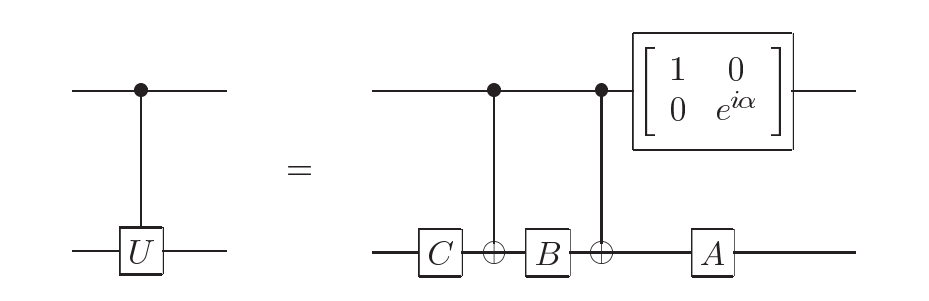
\includegraphics[width=\textwidth]{construct}
\end{figure}

We can also have gates that have more than a single qubit as their control qubit. A controlled $U$ gate with $n$ controls is represented as $C^n(U)$

\begin{exercise}
Prove that a $C^2(U)$ gate (for any single qubit unitary $U$) can be
constructed using at most eight one-qubit gates, and six CNOT gates
\end{exercise}

A lot can be said about multi qubit gates but essentially the main point is that it can be proven that any unitary operation on multiple qubits can be achieved upto arbitrary accuracy using hadamard, phase, CNOT, and $\pi/8$ gates. The proof is a bit involved and we skip it but the main idea is that any unitary operation on multiple qubits can be expressed as a product of unitary operators that operate on two or less qubits. Thus if we show that we can construct any unitary operator acting on two or less qubits we are done. It is then proven that single qubit gates with CNOT gates are sufficient to implement any arbitary gate operating on two qubits. Finally we have to show that any single qubit gate can be approximated using some fixed universal gates that we mentioned above. Although it is theoretically proven implementing everything that we have discussed in practice seems quite complicated and this is one of the main challenges that physicists and computer scientists have been working on in order to bring quantum computation to fruition.

We now move onto actually discussing and talking about some quantum algorithms. We will begin with some simple quantum algorithms and make our way towards Quantum Fourier Transform and Quantum Search based algorithms.
\clearpage
\part{Applications and Algorithms}
\chapter{Superdense Coding}
The main question that we seek to answer in this section is that can we transmit more than a single classical bit on information using a single qubit? Intuitively it may seem so and this is infact true as we will see. However simply transferring a single qubit does not work because measurement collapses the qubit. Instead we will be using the properties of the four possible EPR pairs which we describe below.

\begin{figure}[htp]
    \centering
    \caption{The setup of superdense coding with Alice and Bob each possessing one qubit which are entangled}
    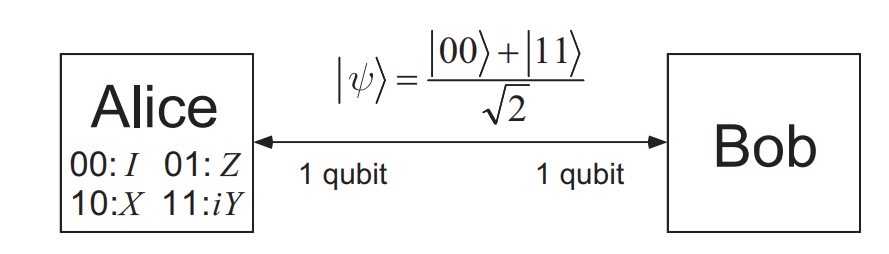
\includegraphics[width=\textwidth]{superdense}
\end{figure}

The EPR pairs or the bell states refer to the four following states comprising of two qubits that are entangled with each other.
$$ \frac{\ket{00} + \ket{11}}{\sqrt{2}}, \frac{\ket{00} - \ket{11}}{\sqrt{2}}, \frac{\ket{10} + \ket{01}}{\sqrt{2}}, \frac{\ket{01} - \ket{10}}{\sqrt{2}}$$

The main idea is that we will use the entanglement of the two qubits in one of these states to transfer two bits of information by simply transferring one bit.
Suppose Alice wants to send Bob two classical bits of information. To do so using superdense coding, an external party will first prepare the state
$$ \ket{\psi} = \frac{\ket{00} + \ket{11}}{\sqrt{2}} $$
and he will then give the first qubit to Alice and the second to Bob.
If Alice wants to send the information $00$ she will do nothing and pass her qubit to Bob.
If she wants to send $01$ then she applies the phase flip gate $Z$, if she wants to send $10$ she applies the quantum NOT gate $X$ to her qubit, if she wants to send $11$ she applies the $iY$ gate. The final state of the entangled qubits corresponding to the information she wants to send is:
$$ 00: \ket{\psi} = \frac{\ket{00} + \ket{11}}{\sqrt{2}}$$
$$ 01: \ket{\psi} = \frac{\ket{00} - \ket{11}}{\sqrt{2}} $$
$$ 10: \ket{\psi} = \frac{\ket{10} + \ket{01}}{\sqrt{2}}$$
$$ 11:  \frac{\ket{01} - \ket{10}}{\sqrt{2}} $$

Notice that all four of these states form a basis and thus when Alice passes her qubit to Bob then Bob can find out which state he got by simply measuring with respect to this basis to figure out which basis vector he had received.

\begin{exercise}
Specify which measurement operators Bob should use to figure out the two classical bits that Alice wanted to send him
\end{exercise}

Notice that this process did involve two qubits but Alice had to send only one qubit. The entanglement of the two qubits allowed Bob to figure out two classical bits of information on transfer of a single qubit.

Let's now look at the reverse, can we transmit a qubit by sending only classical information?

\section{Quantum Teleportation}

This time we want Alice to send two classical bits of information to "send" a qubit. This seems a bit complicated as a qubit is determined by one of it's coefficients along a computational basis. This after taking out a global phase factor can be a real number and so may have a lot of digits in it's expansion and it seems counter intuitive that two classical bits can transmit this information.

However we again leverage the power of entanglement and the EPR pairs. We first let an external agent prepare the first bell state given by
$$ \ket{\beta_{00}} = \frac{\ket{00} + \ket{11}}{\sqrt{2}}$$
We again give the first qubit to Alice and the second to Bob. Now suppose Alice wants to send or teleport the following qubit to Bob.

$$ \ket{\psi} = \alpha\ket{0} + \beta\ket{1}$$

The composite quantum state which we have considering $\ket{\psi}$ will be $$\ket{\psi_{0}} = \ket{\psi}\ket{\beta_{00}}$$

Alice can use the following circuit to convert the composite system of the bell state and this qubit to convert the state into a form that can be used for teleportation. 
\begin{figure}[htp]
    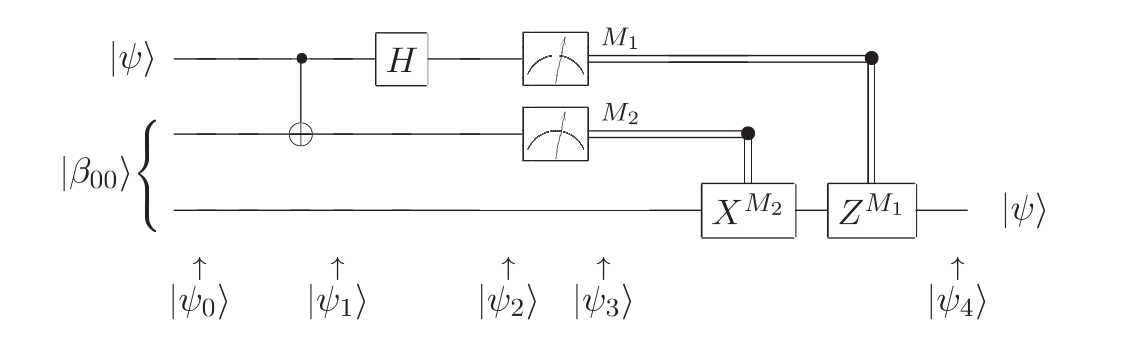
\includegraphics[width=\textwidth]{teleporation}
\end{figure}

Let's go through this circuit one by one. Observe that Alice only has the first two qubits. First a controlled CNOT operation with the qubit corresponding to the state we want to transfer as the control bit is applied.
This results in the state 
$$ \ket{\psi_1} = \frac{\alpha\ket{0}(\ket{00} + \ket{11}) + \beta\ket{1}(\ket{10} + \ket{01})}{\sqrt{2}}$$

Then a Hadamard gate on the first qubit is applied. This results in the net state being (verify that this is indeed the third state)

$$ \ket{\psi_3} = \frac{\ket{00}(\alpha\ket{0} + \beta\ket{1}) + \ket{01}(\alpha\ket{1} + \beta\ket{0}) + \ket{10}(\alpha\ket{0} - \beta\ket{1}) + \ket{11}(\alpha\ket{1} - \beta\ket{0})}{2}$$

Now this state is rather useful for us. Observe that if we measure the first two qubits, depending upon which state the first two qubits collapse into the third qubit will be one of the following states,
$$ \ket{00} : \alpha\ket{0} + \beta\ket{1}$$
$$ \ket{01} : \alpha\ket{1} + \beta\ket{0}$$
$$ \ket{10} : \alpha\ket{0} - \beta\ket{1}$$
$$ \ket{11} : \alpha\ket{1} - \beta\ket{0}$$

Thus if Alice measures the first two qubits that she possesses, depending on her result, the third qubit with Bob will change into one of the four states. If Alice passes her measurement result information (which is given in the form of two classical bits) to Bob, Bob can fix his state to obtain the state $\ket{\psi}$ back. Verify from the diagram that applying that the operations $X$ and $Z$ do indeed result in the original state reverting. For instance if the result was $11$ then Bob will apply both the $X$ and $Z$ gates while if it was $01$ then only the Z gate is applied. Thus using the EPR pair we can achieve quantum teleportation.


An important point to note here is that Quantum Teleportation does not violate the quantum no cloning theorem. Observe that we did not copy the original state to be transferred as the original state transformed into a different state losing it's initial properties. In a sense we have transferred the information, not copied it.
\section{Deutsch-Jozsa Algorithm}

\subsection{Motivation}

One interesting property of quantum circuits that we want to leverage is parallelism. This follows directly from the principle of superposition. To make it a bit more clear let us consider a black box that allows us to compute a function $f: \{0, 1\}^n \to \{0, 1\}$. We however need a place to store the result. We thus want to have a function that achieves the following operation for us,
$$ \ket{x,y} \to \ket{x, f(x)\oplus y}$$
This can be achieved with a unitary operator $U_f$. The process for constructing such an oracle would be to take the classical circuit for computing $f(x)$ and use quantum equivalents of the gates used in this circuit. Leaving aside this implementational detail we observe that if we pass in a superposition of states in $x$ in principle we can obtain multiple values of the function in a single pass.
For instance consider the simple case of $n = 1$ and suppose that
$$ x = \frac{\ket{0} + \ket{1}}{\sqrt{2}}$$

\begin{figure}[htp]
    \centering
    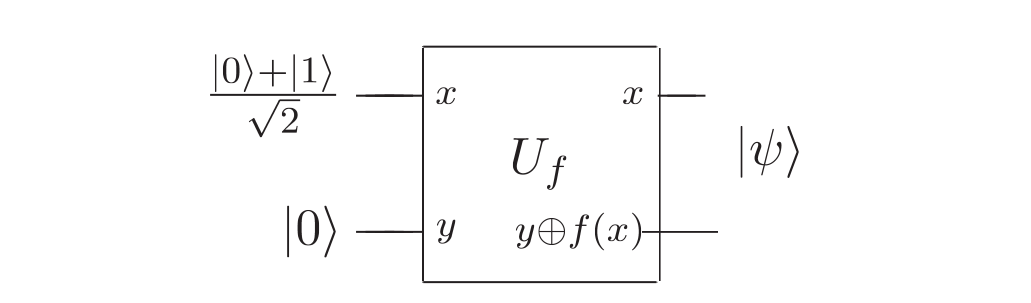
\includegraphics[width=\textwidth]{deutsch}
\end{figure}

Then the final state $\ket{\psi}$ would then be simply
$$\ket{\psi} = \frac{\ket{0, f(0)} + \ket{1, f(1)}}{\sqrt{2}}$$
This means that we have obtained two values of the function $f(x)$ by evaluating our quantum circuit just once. But unfortunately this state is a superposition. We cannot obtain both the values as measurement once collapses this state. What we therefore desire is to use this power of superposition to obtain non trivial values that would normally require us to compute the classical circuit multiple times. The Deustch Algorithm allows to find $f(0) \oplus f(1)$ by just evaluating the circuit once.

\subsection{Deustch Algorithm}

In order to obtain $f(0) \oplus f(1)$ we will use the oracle after applying the hadamard gate on the input qubits $\ket{0}$ and $\ket{1}$. This gives us a form that becomes useful in determining $f(0) \oplus f(1)$ as we will see.

Refer to the figure on the next page to see the circuit we will be implementing. 
The state $\ket{\psi_1} $ is given by
$$ \ket{\psi_1} = \frac{\ket{00} - \ket{01} + \ket{10} - \ket{11}}{2} = 
\left[\frac{\ket{0} + \ket{1}}{\sqrt{2}} \right] \left[\frac{\left{0} - \ket{1}}{\sqrt{2}}\right]$$

The state $\ket{\psi_2}$ after applying the oracle can be written in the following form 
$$\ket{\psi_2} = \pm \left[ \frac{\ket{0} + \ket{1}}{\sqrt{2}}\right]\left[\frac{\ket{0} - \ket{1}}{\sqrt{2}} \right]$$ if $f(0) = f(1)$ otherwise $$\ket{\psi_2} = \pm \left[ \frac{\ket{0} - \ket{1}}{\sqrt{2}}\right]\left[\frac{\ket{0} - \ket{1}}{\sqrt{2}} \right]$$

Observe that by applying the hadamard on the first qubit and observing that $\ket{f(0) \oplus f(1)} = \ket{0}$ if $f(0) = f(1)$ and $\ket{1}$ otherwise gives the state $\ket{\psi_3}$ as 
$$ \ket{\psi_3} = \ket{f(0) \oplus f(1)} \left[\frac{\ket{0} - \ket{1}}{\sqrt{2}} \right]$$

Now simply measuring the first qubit allows us to find $f(0) \oplus f(1)$ in one single evaluation of the quantum circuit. This is Deustch's algorithm.
\begin{figure}[htp]
    \centering
    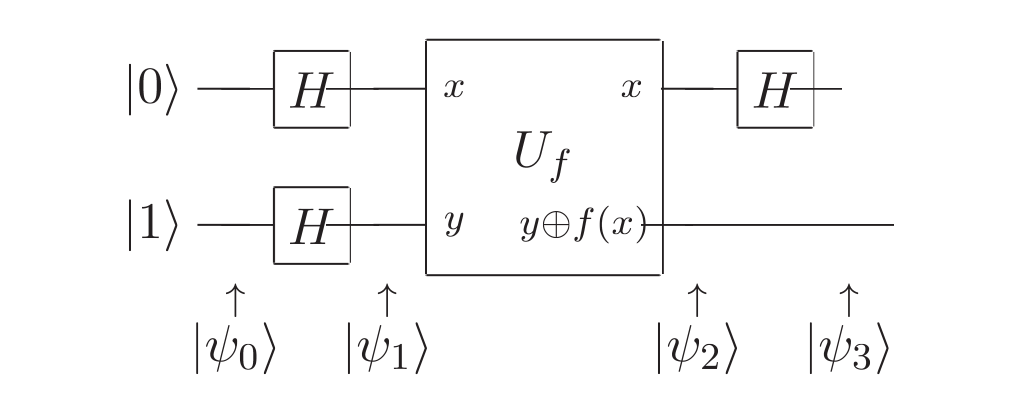
\includegraphics[width=\textwidth]{deutschcircuit}
\end{figure}

\subsection{The Deutsch-Jozsa Algorithm}

\begin{figure}[htp]
    \centering
    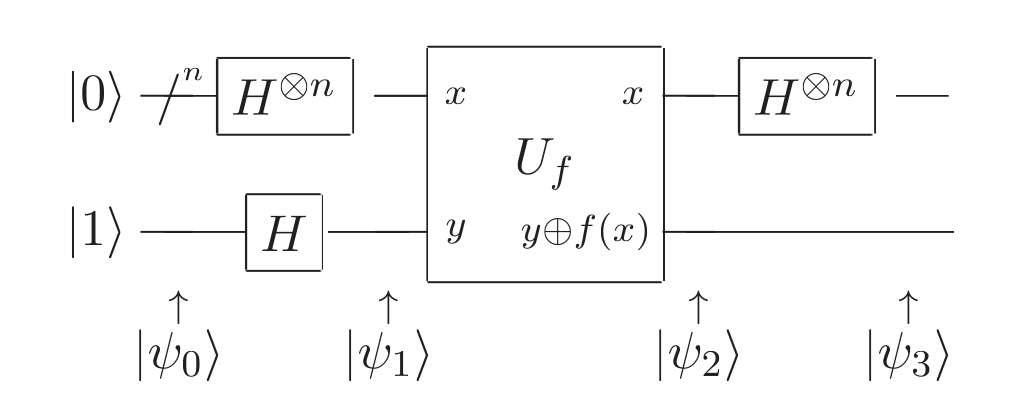
\includegraphics[width=\textwidth]{joschza}
\end{figure}

Deutsch Algorithm is a special case of the more specific Deutsch-Jozsa Algorithm. Consider the following problem which can be formulated as a game.Alice, in Amsterdam, selects a number x from $0$ to $2^n − 1$, and mails it in a letter to Bob, in Boston. Bob calculates some function
$f(x)$ and replies with the result, which is either $0$ or $1$. Now, Bob has promised to use
a function f which is of one of two kinds; either $f(x)$ is constant for all values of $x$,
or else $f(x)$ is balanced, that is, equal to $1$ for exactly half of all the possible $x$, and $0$
for the other half. Alice’s goal is to determine with certainty whether Bob has chosen a
constant or a balanced function, corresponding with him as little as possible. Classically clearly we need atleast $2^{n-1} + 1$ classical bits to resolve this. Can we do better using quantum algorithms?

It turns out we need to evaluate the oracle only once to solve this. Notice that the previous algorithm solved exactly this for the case $n=1$. Our modified oracle takes in $n$ qubits and outputs the value of $f(x)$ in the target register which we set to $\ket{1}$ initially. The circuit is shown in the previous page.

Observe that we can write $\ket{\psi_1}$ as 
$$\ket{\psi_1} = \frac{\sum_{x \in \{0, 1\}^n} \ket{x} }{\sqrt{2^n}} \left[ \frac{\ket{0} - \ket{1}}{\sqrt{2}} \right]$$

$\ket{\psi_2}$ then becomes 
$$\ket{\psi_2} = \frac{\sum_{x \in \{0, 1\}^n} (-1)^{f(x)}\ket{x} }{\sqrt{2^n}} \left[ \frac{\ket{0} - \ket{1}}{\sqrt{2}} \right]$$

Finally we apply the n gate hadamard on the first register of $n$ qubits. These qubits are already in superposition so it seems a bit complex to apply it on all of them. We can however write it as a double sum.

\begin{exercise}
Prove that $$H^{\otimes n} \ket{x_1, x_2 \cdots x_n} = \frac{\sum_{z_1, z_{2}, \cdots z_n}(-1)^{x_{1}z_{1} + x_{2}z{2} \cdots x_{n}z{n}}\ket{z_1, z_2 \cdots z_n}}{\sqrt{2^n}}$$
\end{exercise}

The above can be written simply in the form 
 $$H^{\otimes n} \ket{x} = \frac{\sum_{z}(-1)^{x.z}\ket{z}}{\sqrt{2^n}}$$ 
where $x.z$ is the bitwise product modulo 2.

Thus we can write $\ket{\psi_3}$ as
$$\ket{\psi_3} = \sum_z \sum_x \frac{\sum_{z}(-1)^{x.z + f(x)}\ket{z}}{\sqrt{2^n}}\left[\frac{\ket{0} - \ket{1}}{\sqrt{2}} \right]$$

Now suppose $f(x)$ is constant. Then we can see that the coefficient of $\ket{0}^{\otimes n}$ is either $+1$ or $-1$ depending on $f(x)$. But this means that if we measure the first $n$ qubits in the register we will obtain $\ket{0}^{\otimes n}$ with certainty as our state vector is of unit length and so the other terms have amplitude $0$. Conversely if $f(x)$ is balanced the coefficient of  $\ket{0}^{\otimes n}$ is $0$. Thus is we measure the qubits in the first register and if we obtain $\ket{0}^{\otimes n}$  we see that $f(x)$ is constant and otherwise it is balanced.

Thus using only one pass through the oracle we can solve this problem. This is far far better than the classical case where we need to evaluate the function at $2^{n-1} + 1$ values. This sums up the Deutsch-Jozsa Algorithm.
\chapter{Quantum Fourier Transform}

\section{Introduction to the Discrete Quantum Fourier Transform}

The discrete fourier transform on a vector $x = \left( x_0, x_1 \cdots x_{n-1} \right)$ is given by the vector $y = \left(y_{0}, y_1 \cdots y_{n-1} \right)$ where we have
$$ y_j = \frac{\sum_{k=0}^{n-1} x_k \exp(\frac{2\pi ijk}{n})}{\sqrt{n}}$$

Analogously we can define the discrete fourier transform of our quantum hilbert space of $n$ qubits by the linear operator that takes our basis states $\ket{j} \in \{ \ket{0}, \ket{1} \cdots \}$ to the state given by
$$ \ket{j} \to \frac{1}{\sqrt{2^n}}\sum_{k=0}^{n-1} \exp(\frac{2\pi ijk}{n}) \ket{k}} $$

\begin{exercise}
Prove that the above transformation is unitary
\end{exercise}

\begin{exercise}
Prove that the above quantum unitary operation achieves the discrete fourier transform as defined for a sequence/vector as given above.
\end{exercise}

We state the following compact form for the fourier transform for our quantum hilbert space which makes it easier to construct a circuit to achieve the quantum fourier transform. This follows by some basic algebra which we leave as an exercise.

$$ \ket{j_1, j_2 \cdots j_n} \to \frac{\left(\ket{0} + e^{2\pi i0.j_n}\ket{1} \right)\left(\ket{0} + e^{2\pi i0.j_{n-1}j_n}\ket{1} \right) \cdots \left(\ket{0} + e^{2\pi i0.j_{1}j_{2}\cdots j_{n}}\ket{1} \right)}{\sqrt{2^n}}$$

The circuit below computes the quantum fourier transform

\begin{figure}[htp]
    \centering
    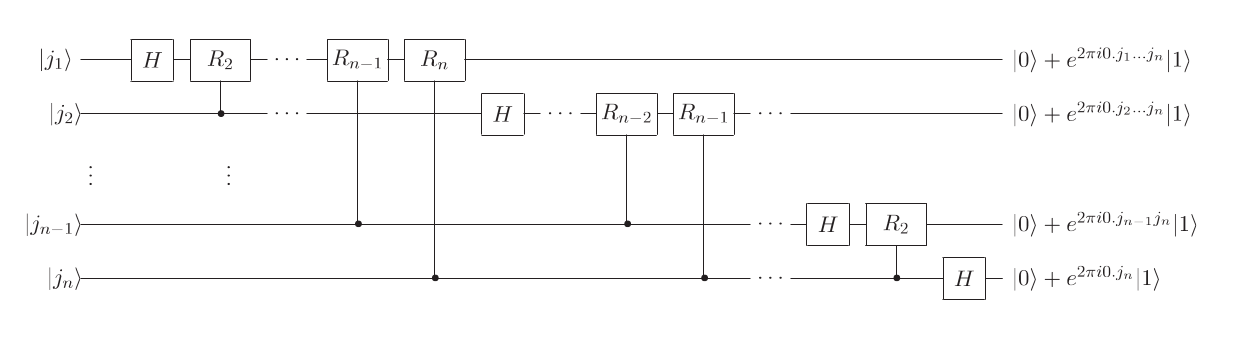
\includegraphics[width=\textwidth]{qft}
\end{figure}

where $R_k$ is defined to be the gate acting on a single qubit given by the matrix
$$R_k = \begin{bmatrix}
1 & 0 \\
0 & e^{2\pi i/2^k} 
\end{bmatrix}$$

To see why observe that the hadamard gate on a qubit $\ket{j_1}$ changes it to
$$\ket{j_1} \to \frac{\left( \ket{0} + e^{2\pi 0.j_1}\ket{1} \right)}{\sqrt{2}}$$

Successive applications of the controlled $R$ gates then finally take $\ket{j_1}$ to 
$$\ket{j_1} \to \frac{\left( \ket{0} + e^{2\pi 0.j_{1}j_{2}\cdots j_{n}}\ket{1} \right)}{\sqrt{2}}$$

We repeat the same process with the other input bits and then take their tensor product to get the form of quantum fourier transform that we obtained above. Notice that we will have to use swap gates (cross over gates that swap qubits) in order to obtain the order given in the compact form above.

Notice that we needed gates in the order of $n^2$ to do the above operation. Thus the Quantum Fourier Transform requires $O(n^2)$ operations to finish where the operation of one single qubit gate is taken as a constant. This is a massive improvement over the classical algorithms which require exponential gates to finish.

Now we will look at some applications of Quantum Fourier Transform, beginning with Phase Estimation.

\section{Phase Estimation}
Using Quantum Fourier Transform we can easily estimate the phase of the eigenvalue of a unitary operator. Recall that unitary operators have eigenvalues whose absolute value is one. Thus for any unitary operator $U$ has it's eigenvalues in the form $e^{i\varphi}$. For now we assume that we have a way of preparing an eigenstate of $U$ $\ket{u}$ with eigenvalue $e^{2\pi i\varphi}$. Thus,
$$ U\ket{u} = e^{2\pi i\varphi}\ket{u}$$
For now suppose that $\varphi$ in binary can be written in the form $0.\varphi_{1}\varphi_{2}\cdots\varphi_{n}$ exactly. That is,
$$\varphi = \sum_{i=1}^{n} \frac{\varphi_{i}}{2^{i}} $$ The following circuit can be used to find $\varphi$

\begin{figure}[htp]
    \centering
    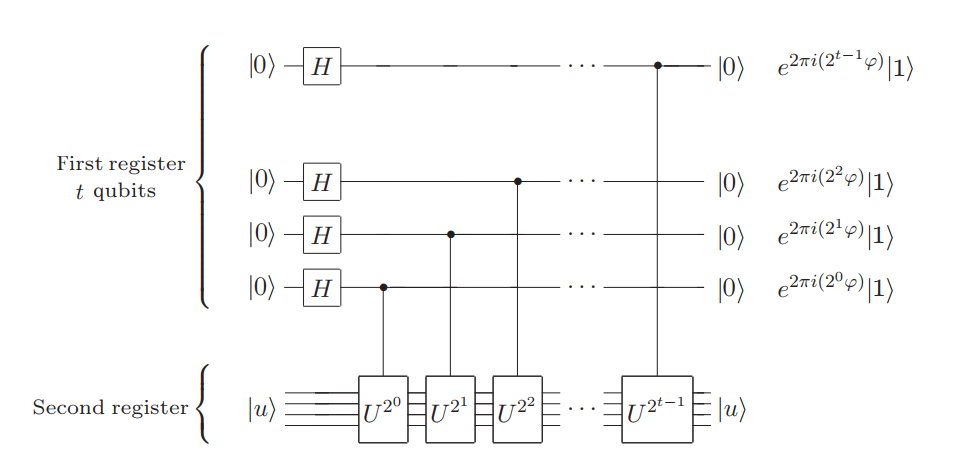
\includegraphics[width=\textwidth]{phase}
\end{figure}

Here we are using the controlled $U^{2^j}$ operation on the second register with the control bits being the t qubits in the control register. Suppose the control qubit is given by $\ket{\psi} = \alpha\ket{0} + \beta\ket{1}$ Observe that when the controlled $U^{2^j}$ operation acts on the second register which is fed in an eigenstate $\ket{u}$ of $U$ it causes the control qubit to change to $\alpha\ket{0} + \beta e^{2\pi i2^{j}\varphi}\ket{1}$. Using this prove the following:
\begin{exercise}
Prove that the final state of the first register in the above circuit will be $$\frac{1}{2^{t/2}}\left( \ket{0} + e^{2\pi i2^{t-1}\varphi}\ket{1} \right)\left( \ket{0} + e^{2\pi i2^{t-2}\varphi}\ket{1} \right) \cdots \left( \ket{0} + e^{2\pi i\varphi}\ket{1} \right) = \sum_{k=1}^{2^t - 1} \frac{1}{2^{t/2}}e^{2\pi i\varphi k}\ket{k}$$
\end{exercise}

Observe that the left hand side of the above final state can be written in the form $$\frac{1}{2^{t/2}}\left( \ket{0} + e^{2\pi i0.\varphi_{t}}\ket{1} \right)\left( \ket{0} + e^{2\pi i0.\varphi_{t-1}\varphi_{t}}\ket{1} \right) \cdots \left( \ket{0} + e^{2\pi 0.\varphi_{1}\varphi_{2}\cdots\varphi_{t}}\ket{1} \right)$$

But this is precisely the result we obtain by taking the quantum fourier transform of the state $\ket{\varphi_{1}\varphi_{2} \cdots \varphi_{t}}$. Thus is we take the inverse fourier transform of the above circuit we will end up with $\ket{\varphi_{1}\varphi_{2} \cdots \varphi_{t}}$ thus giving us the phase.

However in general the phase may not be exactly expressible in $t$ qubits. But it seems intuitive that if use more qubits in the first register then we should be able to get a pretty good estimate of the phase. Indeed this is the case and the following theorem which we state without proof (readers are encouraged to refer to the textbook or wikipedia for details) gives us a quantitative bound on the number of qubits we should use in the first register.

\begin{theorem}
Suppose we desire to obtain the phase $\varphi$ up to an accuracy of $2^{-n}$ with probability of success atleast $1 - \epsilon$ then we should take $t$ qubits in the first register where $t$ is given by
$$ t = n + \left \lceil{\log(2 + \frac{1}{2\epsilon})}\right \rceil $$
\end{theorem}

Notice that after using the above $t$ qubits we should only consider the values in the first $n$ registers. Now that we know how to estimate the phase we can use it to to find the order of a number modulo $N$ and use this to factorise a number. Let's discuss this in detail.

\section{Order Estimation}
The order of a number $x$ modulo $N$ is defined as the least $r$ such that $$ x^r \equiv 1  \mod N$$ Clearly this makes sense only when $\gcd(x, N) = 1$
\begin{exercise}
Prove that $r \leq \phi(N)$
\end{exercise}

On a classical computer it is believed that the order estimation problem is not in $\textbf{P}$ that is there exists no polynomial time algorithm in $L \equiv \left \lceil{ \log(N)} \right \rceil$ which can be used to find the order. We will now use phase estimation to describe such a quantum polynomial algorithm.
For a fixed $x$ let us define a unitary operator $U$ satisfying 
$$U\ket{y} = \ket{xy \Mod{N}}$$ where $y \in \{0, 1\}^L$ with the convention that for $y \geq N$, $\ket{xy \Mod{N}} = y$

\begin{exercise}
Prove that the above operator U is indeed unitary
\end{exercise}
\begin{solution}
Observe that any operator acting on our quantum hilbert space that satisfies the length normalisation condition has to be unitary (why?).
Now observe that the above transformation maps basis vectors to basis vectors and hence must satisfy the length normalisation condition (that is if $\braket{\psi}{\psi} = 1$ then $\braket{U\psi}{U\psi} = 1$) and thus $U$ is unitary.
\end{solution}

Consider the states defined by
$$ \ket{u_s} = \frac{1}{\sqrt{r}} \sum_{k=0}^{r-1} \exp[\frac{-2\pi isk}{r}] \ket{x^k\Mod{N}}$$
\begin{exercise}
Prove that the above states are eigenstates of $U$.
\end{exercise}

We can see that the eigenvalues of the above eigenstate $\ket{u_s}$ will be $\exp(\frac{2\pi is}{r})$. Therefore phase estimation will allow us to find an approximation to $s/r$ upto the number of qubits we desire. Then we will use the continued fractions algorithm to obtain $r$ (more on that later).

This however is not as easy. Firstly we have no way to prepare an eigenstate of $U$. Fortunately we can use the following fact
\begin{exercise}
Prove that $$\frac{1}{\sqrt{r}} \sum_{s=0}^{r-1} \ket{u_s} = \ket{1}$$
\end{exercise}

This is useful because now instead of passing in $\ket{u_s}$ in the second register we can pass in $\ket{1}$. Then by linearity the output after inverse fourier transform will be 
$$ \sum_{s=0}^{r-1} \frac{1}{\sqrt{r}}\ket{\phi_s}\ket{u_s} $$ where $\phi_s$ is an approximation to $s/r$. Now when we start measuring the first register we will finally obtain the binary representation of $s/r$ where $s$ will be a whole number less than $r$ and the probability of $s$ equaling any such number will be the same for all (as the coefficients across the eigenstates are the same). Infact if we use Theorem 10.1 the probability will be modified to become $\left ( 1 -\epsilon \right)/r$.

We will be wanting an accuracy of $2L + 1$ qubits in our estimate as we will see later. Clearly the number of gates needed will be $O(L^2)$ for the inverse fourier transform. For the phase estimation observe that we would also need an efficient way to do controlled $U^{2^j}$ operations. This can be shown to be done with $O(L^3)$ gates using modular exponentation. Thus so far we need $O(L^3)$ gates to perform the phase estimation.
\begin{figure}[htp]
    \centering
    \caption{Circuit for Order Estimation}
    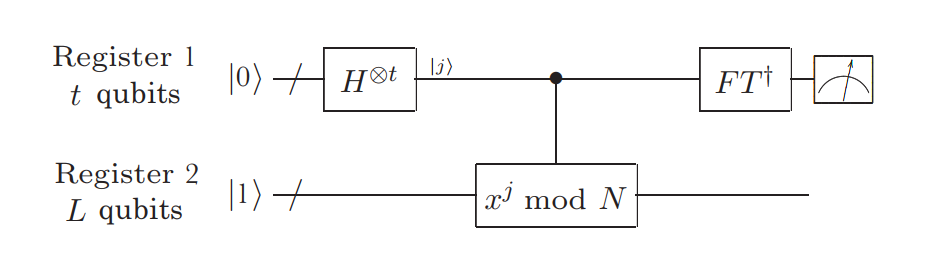
\includegraphics[width=\textwidth]{order}
\end{figure}

Now to extract $r$ from $s/r$ we will use the continued fractions algorithm. The following theorem becomes incredibly useful

\begin{theorem}
Let $s/r$ be a rational number such that for another rational number $\phi$ it satisfies 
$$ |\frac{s}{r} - \phi| \leq \frac{1}{2r^2}$$
Then $s/r$ is a convergent of the continued fractions expansion of $\phi$
\end{theorem}

\begin{exercise}
Prove that the above condition is held for our $\phi$ being the approximation to $s/r$ upto $2L + 1$ digits.
\end{exercise}

Thus taking our estimate $\phi$ and finding it's continued fraction expansion will allow us to evaluate all the convergents of this continued fraction.

As a recap continued fractions allow us to represent any number $x$ in the form $\left[ a_0, a_1, a_2 \cdots \right]$ where 
$$ x = a_0 + \frac{1}{a_1 + \frac{1}{a_2 + \frac{1}{\cdots}}} $$
In the case of rationals this set is finite. The convergent simply corresponds to select a prefix of this set, that is if the representation of the rational was $\left[ a_0, a_1, a_2 \cdots a_M \right]$  then the $mth$ convergent will simply be $\left[ a_0, a_1, a_2 \cdots a_m \right]$ where $m \leq M$.

This process also takes $O(L^3)$ gates and then we can simply evaluate all the candidates for $s/r$. Now as we have an exact value for $r$ we can simply check if this is the order or not. Note that if some value of $r$ does satisfy $x^r \equiv 1 \pmod N$ then it must be the order and not a multiple of it (why?). There could be one issue and and that is if $s$ and $r$ have common factors then the continued fractions algorithm will give us $s'$, $r'$ such that $s'/r'$ = $s/r$. But this isn't an issue because the probability of $s$ and $r$ being coprime is high and so we can simply run the process multiple times until we get the value of $r$ that we seek.

Thus we have found the order of $x$ modulo $N$ using only $O(L^3)$ gates. This we shall see will become very useful in factoring numbers as this is a routine used in Shor's algorithm.

\section{Shor's Algorithm}
\begin{figure}[htp]
    \caption{Circuit for Shor's algorithm}
    \centering
    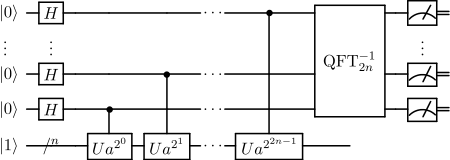
\includegraphics[width=\textwidth]{shor}
\end{figure}
Shor's algorithm for factoring uses the order finding algorithm that we described above to factorise a number. All the other step's in Shor's algorithm can be done using a classical computer efficiently and thus it is the quantum order finding subroutine that is the main component of Shor's algorithm.

We can reduce the factoring problem to the order finding problem. We will show this equivalence using a few theorems. First consider the following interesting theorem

\begin{theorem}
Suppose $N$ is an $L$ bit composite number, and $x$ is a non-trivial solution to the equation $x^2 \equiv  1 \pmod N$ in the range $1 \leq x \leq N$, that is, neither $x \equiv 1  \pmod N$ nor $x \equiv N - 1 \pmod N$. Then at least one of $\gcd(x − 1, N)$ and $\gcd(x + 1, N)$ is a non-trivial factor of $n$ that can be computed using $O(L^3)$ operations.
\end{theorem}
\begin{proof}
Left as exercise (hint: consider the negation and proceed by contradiction)
\end{proof}

Now suppose we have that $y$ is coprime to $N$ where $ 1 \leq y \leq N$ (else their greatest common divisor will be a divisor of $N$ thus giving us a factor and solving the factoring problem). Suppose the order of $y$ modulo $N$ is even and also satisfies $y^{r/2} \not\equiv -1 \pmod N$. Then we can set $x = y^{r/2}$ in the theorem above and so we can simply use this value to find a non trivial factor of $N$. This is the basic idea of Shor's algorithm. However we need to ensure the above two conditions. We can get a bound on the probability of this occurring and thus by repeating the process a couple of times we can with high probability get a factor. Notice that this is true assuming that the number is composite.

The following theorem gives a bound on the above conditions holding whose proof we omit as it involves generators and group theory.

\begin{theorem}
Suppose $N = p_1^{\alpha_{1}}p_2^{\alpha_{2}} \cdots p_m^{\alpha_m}$ is the prime factorization of an odd composite
positive integer. Let $x$ be an integer chosen uniformly at random, subject to the
requirements that $1 \leq x\leq N - 1$ and $x$ is co-prime to $N$. Let $r$ be the order of
$x$ modulo $N$. Then
$p(r$ is even and $x^{r/2} \equiv − 1 \pmod N ) \geq 1 - \frac{1}{2^m}$
\end{theorem}

Thus the probability of the above condition being satisfied increases as the number of distinct primes dividing our numbers increases. Thus by repeated applications we can ensure that our algorithm suceeds.\\

The summary of the algorithms is as follows:

Input: A composite number $N$
\\
Output: A non trivial factor of $N$
\\
Complexity: $O(\log^3 N)$, succeeds with probability $O(1)$\\
Steps:
\\
1. If $N$ is even return 2\\
2. Else take $x$ satisfying $1 \leq x \leq N-1$. If $\gcd(x, N)$ is not $1$ then return $\gcd(x, N)$\\
3. Else run the order finding algorithm to find the order $r$ of $x$ modulo $N$\\
4. Check if $r$ is even and $x^{r/2} \neq -1 \pmod N$. If this is satisfied compute $\gcd(x^{r/2} - 1, N)$ and $\gcd(x^{r/2} + 1, N)$ and return whichever of them is not equal to 1. If this is not satisfied the algorithm does not succeed.
\\\\
To ensure high probability of success we will run the algorithm multiple times.
This sums up Shor's algorithm and the usage of Quantum Fourier Transform. Quantum Fourier Transform can be used for various other applications like period estimation, discrete logarithm and a class of problems known as the hidden subgroup problem. The reader is encouraged to go through the textbook to study these topics in depth. Now we shall see how Quantum Search can be achieved using Grover's algorithm.
\clearpage
\chapter{Quantum Search Algorithms}

\section{Introduction}
Now we will look at another classical computing task that can be speeded up using the superposition principle. Our goal is to solve the needle in a haystack problem where we have to search for an element that satisfies a particular property that lies in a haystack of $N$ elements. Classically it seems that since this element can be any one of those $N$ elements it will take $O(N)$ steps to do this task. However the quantum algorithm, Grover's algorithm allows us to do this $O(\sqrt{N}$. Let us investigate this in detail by formulating the problem first.
\\\\
Suppose $f(x)$ is a function from $\{0, 1 \cdots, N-1\}$ to $\{0, 1\}$ Only for one value $a$, $f(a) = 1$. We seek to find this $a$. Also assume that $N = 2^n$. This way we can work with $n$ qubits (if $N$ is not of this form we can add extra elements to ensure this). Grover's algorithm involves using rotations in a 2D subspace so that this speedup ends up working.

\section{Grover's Algorithm}

Before we discuss the specifics, let us go through the main idea. Let us define two new state vectors:
$$\ket{\psi_0} = \sum_{i=0}^{N - 1} \frac{\ket{i}}{\sqrt{N}}$$ 
$$\ket{e} = \sum_{i = 0, i \neq a}^{N-1} \frac{\ket{i}}{\sqrt{N-1}}$$

Our goal is to ensure that we obtain $\ket{a}$ in the end. Notice that $$\ket{\psi_0} = \frac{\sqrt{N-1}\ket{e} + \ket{a}}{\sqrt{N}}$$ Thus $\ket{\psi_0}$ lies in the subspace spanned by $\ket{e}$ and $\ket{a}$ The coefficient of $\ket{e}$ is in general far greater than that of $\ket{a}$. Thus $\ket{\psi_0}$ will be closer to $\ket{e}$ than $\ket{a}$. Diagrammatically this can be represented as follows:
\begin{figure}[htp]
    \centering
    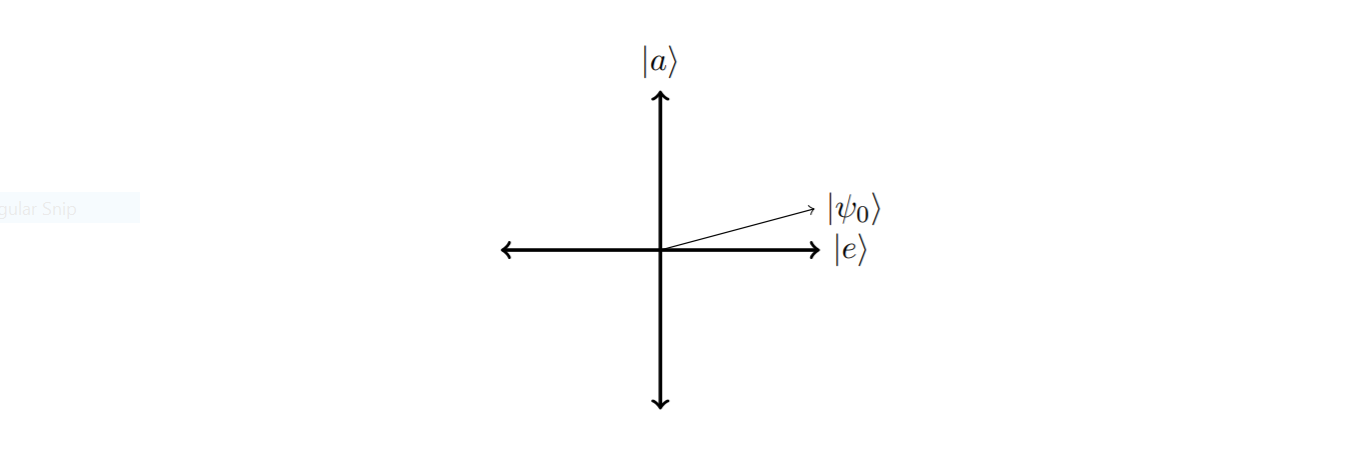
\includegraphics[width=\textwidth]{twod}
\end{figure}

What we aim to do is take a vector $\ket{\psi}$ which will be initially equal to $\ket{\psi_0}$ and rotate it so that it ends up getting close to $\ket{a}$. For this what we would like to do is first reflect $\ket{\psi}$ about $\ket{e}$ and then about $\ket{\psi_0}$. Two reflections simultaneously correspond to a rotation. Reflecting about $\ket{e}$ can be done by considering an oracle that performs the operation
$$ \ket{x} \to (-1)^{f(x)}\ket{x}$$
Notice that we used a similar oracle in Deustch-Josza algoritm. Let us call this operation $O$. The way to achieve this is to take an oracle that performs the operation
$$\ket{x}\ket{y} \to \ket{x}\ket{y \oplus f(x)}$$
The construction of this oracle was described in the section on the Deustch-Josza algoritm. Let $\ket{y} = \frac{\ket{0} - \ket{1}}{\sqrt{2}}$
If $x = a$ then the oracle will perform the following operation
$$\ket{x}\ket{y} \to -\ket{x}\ket{y}$$ and for every other $x$ as $f(x) = 0$ it will preserver the state. Thus using such an oracle and simply ignoring the $\ket{y}$ qubit will allow us to get the behaviour we desire.
Now when this operation is applied on any $\ket{\psi}$ only the component along $\ket{a}$ will be flipped and the rest will remain the same. This achieves reflection about $\ket{e}$. To reflect about $\ket{\psi_0}$ we would like to use the following result that you have to prove:
\begin{exercise}
Prove that the following unitary operation $U = 2\ket{\psi}\bra{\psi} - I$ achieves reflection about the state vector $\ket{\psi}$ (Hint: take any vector in the hilbert space and write it in terms of $\ket{\psi}$ and the bases of the subspace orthogonal to  $\ket{\psi}$)
\end{exercise}

We define the Grover Operator $G$ as $$G = (2\ket{\psi_0}\bra{\psi_0} - I)O$$ This operator first reflects about $\ket{e}$ and then about $\ket{\psi_0}$
\begin{figure}[htp]
    \caption{Result after applying Grover once}
    \centering
    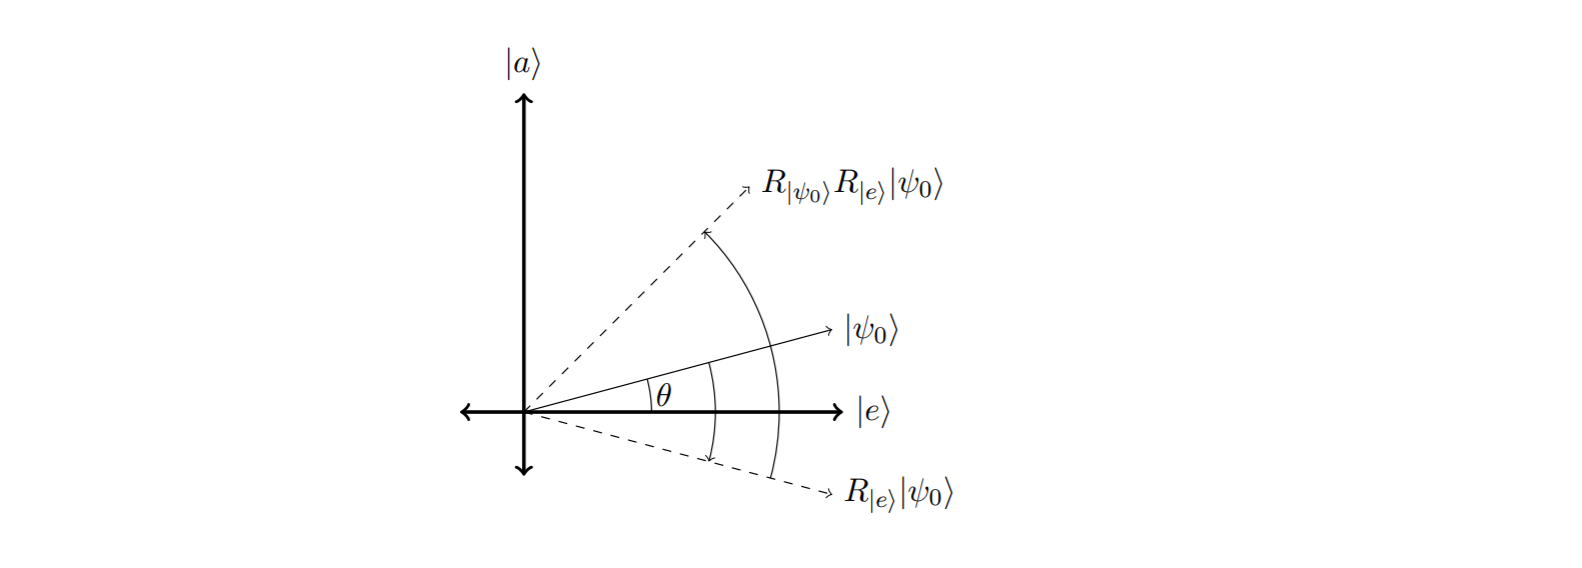
\includegraphics[width=\textwidth]{grover}
\end{figure}
Let $\psi_{0}$ make an angle $\theta$ with $\ket{e}$ in the two dimensional subspace. Then it follows that $\sin(\theta) = \frac{1}{\sqrt{N}}$. The following exercise will allow you to see how successfully applying $G$ changes our state vector which was initially $\ket{\psi_0}$

\begin{exercise}
Prove by induction that 
$$G^k \ket{\psi_0} = \cos((2k+1)\theta)\ket{e} + \sin((2k+1)\theta)\ket{a}$$
\end{exercise}

Thus applying $G$ successively on $\ket{\psi_0}$ rotates the vector by an angle $2\theta$. We can continue applying this to $\ket{\psi}$ until the angle between $\ket{\psi}$ and $\ket{a}$ will be $\leq \theta$. Then the probability of collapsing to $\ket{a}$ will be $\geq \cos(\theta) = \frac{\sqrt{N-1}}{\sqrt{N}}$. For large $N$ this will be very accurate.
How many operations of $G$ do we need though? Clearly we require $\left[ \frac{\pi}{4\theta} \right]$ applications of $G$.
Notice that $\theta \geq \sin(\theta) = \frac{1}{\sqrt{N}}$ and so 
$$\left[ \frac{\pi}{4\theta} \right] \leq \frac{\pi \sqrt{N}}{4}$$
Thus we need only $O(\sqrt{N})$ operations to achieve the task with probability $\geq \frac{\sqrt{N-1}}{\sqrt{N}}$\\\\

Thus the algorithm may be summarised as follows:\\

Algorithm: Grover's Search Algorithm\\
Input: An oracle that does the transformation $$ \ket{x} \to (-1)^{f(x)}\ket{x}$$\\
Output: The only $a$ satisfying $f(a) = 1$ with probability of success $\geq \frac{\sqrt{N-1}}{\sqrt{N}}$\\
Procedure:\\
1. Create the state $\psi_0$ by applying $H^{\otimes n}\ket{0}$\\
2. Apply the Grover operation $G = (2\ket{\psi_0}\bra{\psi_0} - I)O$ $\left[ \frac{\pi}{4\theta} \right]$ times\\
3. Measure the $n$ qubits to get $a$\\

This case of Grover's algorithm was defined when we had to search for only one element. We can modify it when multiple $x$ satisfied $f(x) = 1$ in which case we would have obtained different values of $x$ as the output (only one output per iteration of the algorithm). This modification is left as an exercise. You may want to change the two vectors that we took as the basis of the two dimension subspace over which we worked. The algorithm in this case will be $O(\sqrt{N/M})$

With this we have successfully described Grover's algorithm for searching. Although the speedup is not as significant as that in fourier transform or factoring the gains are significant. Grover's algorithm can be useful in solving $\textbf{NP Hard}$ problems by allowing us to search through the search space more quickly.

One question that may come to our minds is whether we can hope for a more significant speedup by modifying our algorithm. It has been however proven that any quantum search algorithm for the general case would still require $O(\sqrt{N})$ operations to terminate and thus Grover's algorithm is an asymptotically optimal algorithm.


\chapter{Conclusion}
With this we have come to the end of the report. The report mainly focused on the basics of quantum computation where we began from elementary linear algebra and built our way towards the basics of quantum mechanics, computer science, quantum circuits and eventually made it to some notable quantum algorithms and their applications. The report was in no way exhaustive and it is recommended that readers consult Nielsen and Chuang along the way. It is also essential to note that although we have described everything from a theoretical perspective a lot of work is still going on regarding how to put everything into practice as making hardware that is natively suited for quantum computing has proven to be a challenge. We are hopeful that in the coming years advances in technology will allow the power of quantum computation to come to fruition.
\end{document}
